% Options for packages loaded elsewhere
\PassOptionsToPackage{unicode}{hyperref}
\PassOptionsToPackage{hyphens}{url}
\PassOptionsToPackage{dvipsnames,svgnames,x11names}{xcolor}
%
\documentclass[
  number,
  preprint]{elsarticle}

\usepackage{amsmath,amssymb}
\usepackage{iftex}
\ifPDFTeX
  \usepackage[T1]{fontenc}
  \usepackage[utf8]{inputenc}
  \usepackage{textcomp} % provide euro and other symbols
\else % if luatex or xetex
  \usepackage{unicode-math}
  \defaultfontfeatures{Scale=MatchLowercase}
  \defaultfontfeatures[\rmfamily]{Ligatures=TeX,Scale=1}
\fi
\usepackage{lmodern}
\ifPDFTeX\else  
    % xetex/luatex font selection
\fi
% Use upquote if available, for straight quotes in verbatim environments
\IfFileExists{upquote.sty}{\usepackage{upquote}}{}
\IfFileExists{microtype.sty}{% use microtype if available
  \usepackage[]{microtype}
  \UseMicrotypeSet[protrusion]{basicmath} % disable protrusion for tt fonts
}{}
\makeatletter
\@ifundefined{KOMAClassName}{% if non-KOMA class
  \IfFileExists{parskip.sty}{%
    \usepackage{parskip}
  }{% else
    \setlength{\parindent}{0pt}
    \setlength{\parskip}{6pt plus 2pt minus 1pt}}
}{% if KOMA class
  \KOMAoptions{parskip=half}}
\makeatother
\usepackage{xcolor}
\setlength{\emergencystretch}{3em} % prevent overfull lines
\setcounter{secnumdepth}{5}
% Make \paragraph and \subparagraph free-standing
\makeatletter
\ifx\paragraph\undefined\else
  \let\oldparagraph\paragraph
  \renewcommand{\paragraph}{
    \@ifstar
      \xxxParagraphStar
      \xxxParagraphNoStar
  }
  \newcommand{\xxxParagraphStar}[1]{\oldparagraph*{#1}\mbox{}}
  \newcommand{\xxxParagraphNoStar}[1]{\oldparagraph{#1}\mbox{}}
\fi
\ifx\subparagraph\undefined\else
  \let\oldsubparagraph\subparagraph
  \renewcommand{\subparagraph}{
    \@ifstar
      \xxxSubParagraphStar
      \xxxSubParagraphNoStar
  }
  \newcommand{\xxxSubParagraphStar}[1]{\oldsubparagraph*{#1}\mbox{}}
  \newcommand{\xxxSubParagraphNoStar}[1]{\oldsubparagraph{#1}\mbox{}}
\fi
\makeatother


\providecommand{\tightlist}{%
  \setlength{\itemsep}{0pt}\setlength{\parskip}{0pt}}\usepackage{longtable,booktabs,array}
\usepackage{calc} % for calculating minipage widths
% Correct order of tables after \paragraph or \subparagraph
\usepackage{etoolbox}
\makeatletter
\patchcmd\longtable{\par}{\if@noskipsec\mbox{}\fi\par}{}{}
\makeatother
% Allow footnotes in longtable head/foot
\IfFileExists{footnotehyper.sty}{\usepackage{footnotehyper}}{\usepackage{footnote}}
\makesavenoteenv{longtable}
\usepackage{graphicx}
\makeatletter
\def\maxwidth{\ifdim\Gin@nat@width>\linewidth\linewidth\else\Gin@nat@width\fi}
\def\maxheight{\ifdim\Gin@nat@height>\textheight\textheight\else\Gin@nat@height\fi}
\makeatother
% Scale images if necessary, so that they will not overflow the page
% margins by default, and it is still possible to overwrite the defaults
% using explicit options in \includegraphics[width, height, ...]{}
\setkeys{Gin}{width=\maxwidth,height=\maxheight,keepaspectratio}
% Set default figure placement to htbp
\makeatletter
\def\fps@figure{htbp}
\makeatother

\usepackage{booktabs}
\usepackage{longtable}
\usepackage{array}
\usepackage{multirow}
\usepackage{wrapfig}
\usepackage{float}
\usepackage{colortbl}
\usepackage{pdflscape}
\usepackage{tabu}
\usepackage{threeparttable}
\usepackage{threeparttablex}
\usepackage[normalem]{ulem}
\usepackage{makecell}
\usepackage{xcolor}
\makeatletter
\@ifpackageloaded{caption}{}{\usepackage{caption}}
\AtBeginDocument{%
\ifdefined\contentsname
  \renewcommand*\contentsname{Table of contents}
\else
  \newcommand\contentsname{Table of contents}
\fi
\ifdefined\listfigurename
  \renewcommand*\listfigurename{List of Figures}
\else
  \newcommand\listfigurename{List of Figures}
\fi
\ifdefined\listtablename
  \renewcommand*\listtablename{List of Tables}
\else
  \newcommand\listtablename{List of Tables}
\fi
\ifdefined\figurename
  \renewcommand*\figurename{Figure}
\else
  \newcommand\figurename{Figure}
\fi
\ifdefined\tablename
  \renewcommand*\tablename{Table}
\else
  \newcommand\tablename{Table}
\fi
}
\@ifpackageloaded{float}{}{\usepackage{float}}
\floatstyle{ruled}
\@ifundefined{c@chapter}{\newfloat{codelisting}{h}{lop}}{\newfloat{codelisting}{h}{lop}[chapter]}
\floatname{codelisting}{Listing}
\newcommand*\listoflistings{\listof{codelisting}{List of Listings}}
\makeatother
\makeatletter
\makeatother
\makeatletter
\@ifpackageloaded{caption}{}{\usepackage{caption}}
\@ifpackageloaded{subcaption}{}{\usepackage{subcaption}}
\makeatother
\journal{Health Economics Study Group}

\ifLuaTeX
  \usepackage{selnolig}  % disable illegal ligatures
\fi
\usepackage[]{natbib}
\bibliographystyle{elsarticle-num}
\usepackage{bookmark}

\IfFileExists{xurl.sty}{\usepackage{xurl}}{} % add URL line breaks if available
\urlstyle{same} % disable monospaced font for URLs
\hypersetup{
  pdftitle={Development of a value-based scoring system for the WAItE using the OPUF in a sample of adults},
  pdfkeywords={preference elicitation, quality of life},
  colorlinks=true,
  linkcolor={blue},
  filecolor={Maroon},
  citecolor={Blue},
  urlcolor={Blue},
  pdfcreator={LaTeX via pandoc}}


\setlength{\parindent}{6pt}
\begin{document}

\begin{frontmatter}
\title{Development of a value-based scoring system for the WAItE using
the OPUF in a sample of adults}

\affiliation[1]{organization={Newcastle University, Health Economics
Group},addressline={University, Barras Bridge},city={Newcastle upon
Tyne},postcode={NE1 7RU},postcodesep={}}
\affiliation[2]{organization={Northumbria University, Nursing, Midwifery
and Health},addressline={Ellison Pl},city={Newcastle upon
Tyne},postcode={NE1 8ST},postcodesep={}}

\cortext[cor1]{Corresponding author}
        
\begin{abstract}
\textbf{Background:} Online personal utility functions (OPUF) present a
new method for eliciting preferences. In this study we used the OPUF to
elicit a health state utility value set for the Weight-specific
Adolescent Instrument for Economic-evaluation (WAItE) with a
representative sample of the UK adult population. \textbf{Methods:}
WAItE OPUF survey design was informed by prior qualitative work. The
survey consisted of the WAItE descriptive system, domain weighting,
level rating (per attribute) and a VAS anchoring task. Personal utility
functions were estimated on the individual level for all participants.
Personal utility functions were aggregated and combined with the
anchoring factor to give the social utility function and utility value
set. Preference heterogeneity was assessed using Euclidean distance and
PERMANOVA to explore preference variation within the sample. An
experimental sensitivity analysis dichotomised preference heterogeneity
into anchoring variation and attribute weighting/level rating variation.
\textbf{Results:} A total of 300 participants completed the WAItE OPUF
survey. The sample was broadly representative of the UK adult
population. Participants, on average, took less than 10 minutes to
complete the survey. The most important attributes were tiredness and
unhappiness, while least important attributes were sports and
embarrassment. Social utility values and the anchoring utility value
estimated were comparable to previous studies. Preferences generally
were heterogeneous, especially among different ages. Younger
participants assigned lower utility values to WAItE health states and
provided significantly lower scores on the VAS anchoring task compared
to older participants. \textbf{Conclusion:} This study successfully
elicited health state utility values for the WAItE using the OPUF.
Preference heterogeneity analysis identified differences in preferences
for different age groups and a further valuation study is ongoing to
explore whether this heterogeneity exists between adults and
adolescents.
\end{abstract}





\begin{keyword}
    preference elicitation \sep 
    quality of life
\end{keyword}
\end{frontmatter}
    

\section{Introduction}\label{sec-introduction}

This chapter presents the introduction, methods, results and discussion
from an empirical study developing a utility value set for the WAItE
using online personal utility functions (OPUF) with a representative
sample of UK adults.

\subsection{Compositional preference elicitation
methods}\label{compositional-preference-elicitation-methods}

Preference elicitation methods generally speaking, fall into two
categories: compositional and decompositional
\citep{Keeney1979DecisionsTrade-Offs, Marsh2016MultipleForce, Belton2002MultipleAnalysis}.
That is, methods like DCE, BWS and TTO elicit preference orderings from
individuals for an entire health state (composed of a combination of
attributes and levels) and then responses are decomposed to identify
marginal contributions of each attribute and level in each health state.
Models like multinomial logit, mixed logit and latent class are
frequently used to decompose responses to decompositional preference
elicitation tasks \citep{Hauber2016StatisticalForce}. Coefficients
estimated in these models form the basis of dis/utility values for each
attribute and level in a descriptive system.

Conversely, compositional methods seek to identify preferences for each
attribute weighting and level rating individually for the number of
attributes and levels in a given descriptive system. Therefore,
statistical models to elicit coefficients for each individual attribute
and level are not required and responses to each attribute weighting and
level rating are combined (in addition to an anchoring factor) to yield
dis/utility values for each attribute and level in the descriptive
system. Compositional approaches can take many forms from simple VAS
scores to using semantic categories and ranking methods
\citep{BanaECosta1999TheApplication, Danner2011IntegratingPreferences, Oliveira2018ValuingStates}.
These approaches have been used successfully in multi-criteria decision
analysis (MCDA), but have been used less extensively in the preference
elicitation space. Since the development of the OPUF, compositional
approaches to elicit preferences have become more commonplace and a
number of countries are using the OPUF to elicit value sets specific to
their population \citep{Brodszky2023PCR108States}.

\subsection{From PUF to OPUF}\label{from-puf-to-opuf}

Personal utility functions were first used in the context of preference
elicitation by Devlin et al.~(2019) \citep{Devlin2019AFunctions} to
estimate the feasibility for using this approach to estimate a value set
for the EQ5D-5L. Since the feasibility for the underlying PUF methods
were established, the approach has been expanded by Schneider and
colleagues and converted into an online personal utility functions
(OPUF) survey built initially using RShiny
\citep{Schneider2022TheStates} and subsequently using Javascript
(available \href{https://eq5d5l.me}{here}). Since the development of the
OPUF, a number of descriptive systems and different research teams have
begun utilising this method to elicit value sets
\citep{Bray2024DevelopmentImpairment, Brodszky2023PCR108States}.

\subsection{An overview of the OPUF
structure}\label{an-overview-of-the-opuf-structure}

\subsubsection{Attribute weighting}\label{attribute-weighting}

This section is composed of two parts. First, attribute ranking is
completed where participants identify their most important attribute
(Figure~\ref{fig-importantattribute}). Second, respondents complete the
attribute weighting (swing weighting) where the relative importance of
other attributes is ascertained using their most important attribute as
a reference point (Figure~\ref{fig-swing}). These questions are
presented in Figure~\ref{fig-attribute}.

\begin{figure}

\begin{minipage}{0.50\linewidth}

\centering{

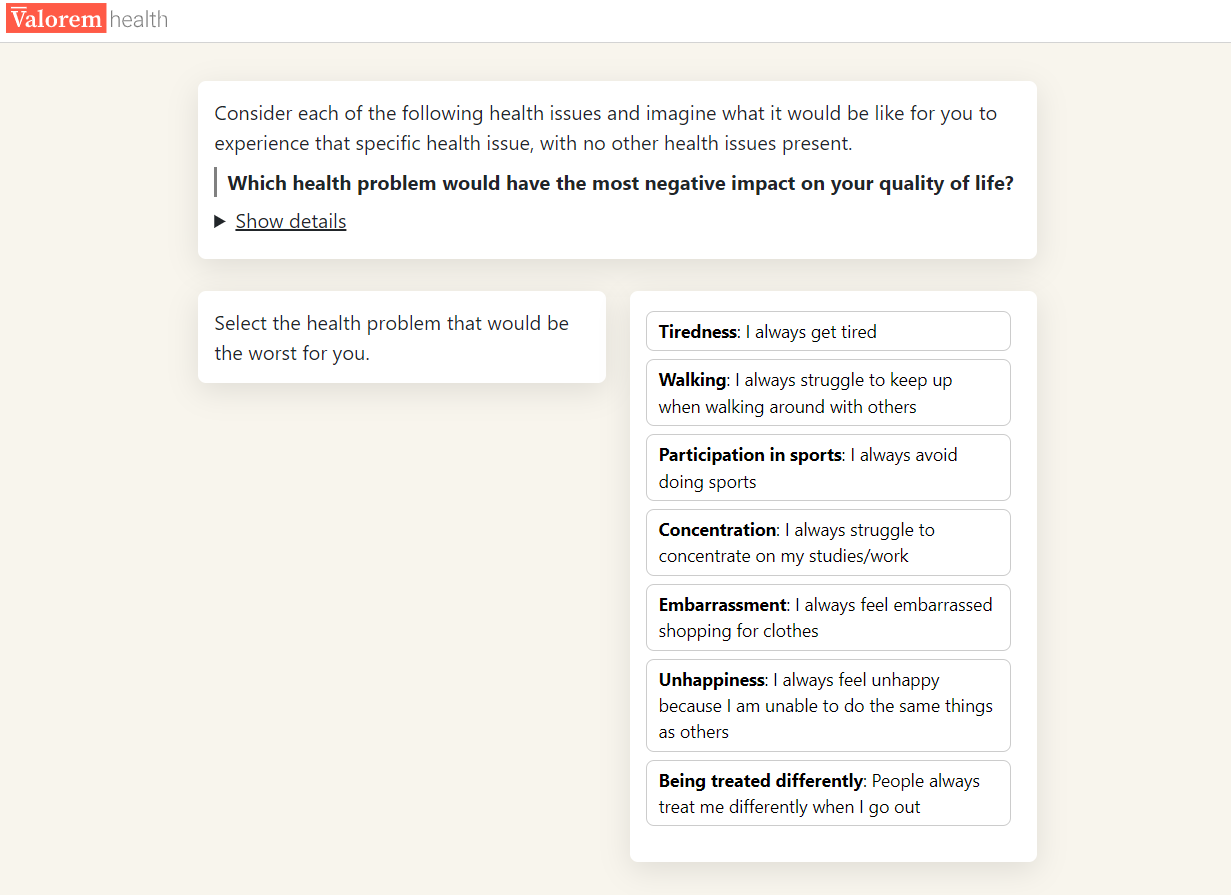
\includegraphics{../../outputs/figures/relative_importance.png}

}

\subcaption{\label{fig-importantattribute}Most important attribute}

\end{minipage}%
%
\begin{minipage}{0.50\linewidth}

\centering{

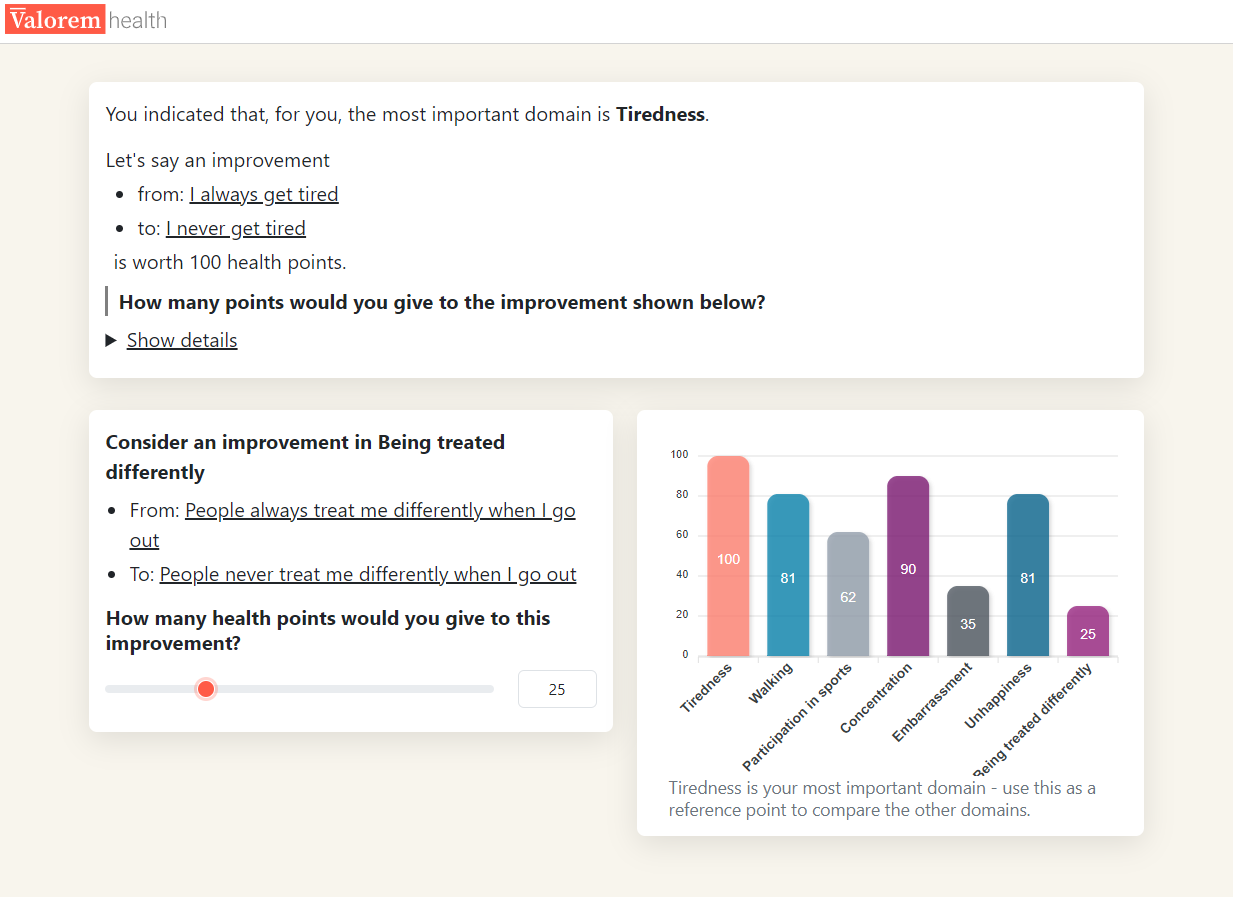
\includegraphics{../../outputs/figures/swing_rating.png}

}

\subcaption{\label{fig-swing}Swing rating}

\end{minipage}%

\caption{\label{fig-attribute}Attribute weighting}

\end{figure}%

\subsubsection{Level ratings}\label{level-ratings}

This element of the OPUF has varied across different iterations of the
survey. Schnieder et al.~(2022) \citep{Schneider2022TheStates} asked
participants to rank the levels within the descriptive system generally
(i.e.~for any given attribute), while other iterations have administered
separate level rating questions for each attribute in the descriptive
system \citep{Bray2024DevelopmentImpairment}. Selection of method
requires a trade-off between participant burden and sensitivity of level
ratings to each attribute. Figure~\ref{fig-level} presents the level
rating question for the tiredness and treated differently attributes of
the WAItE.

\begin{figure}

\begin{minipage}{0.50\linewidth}

\centering{

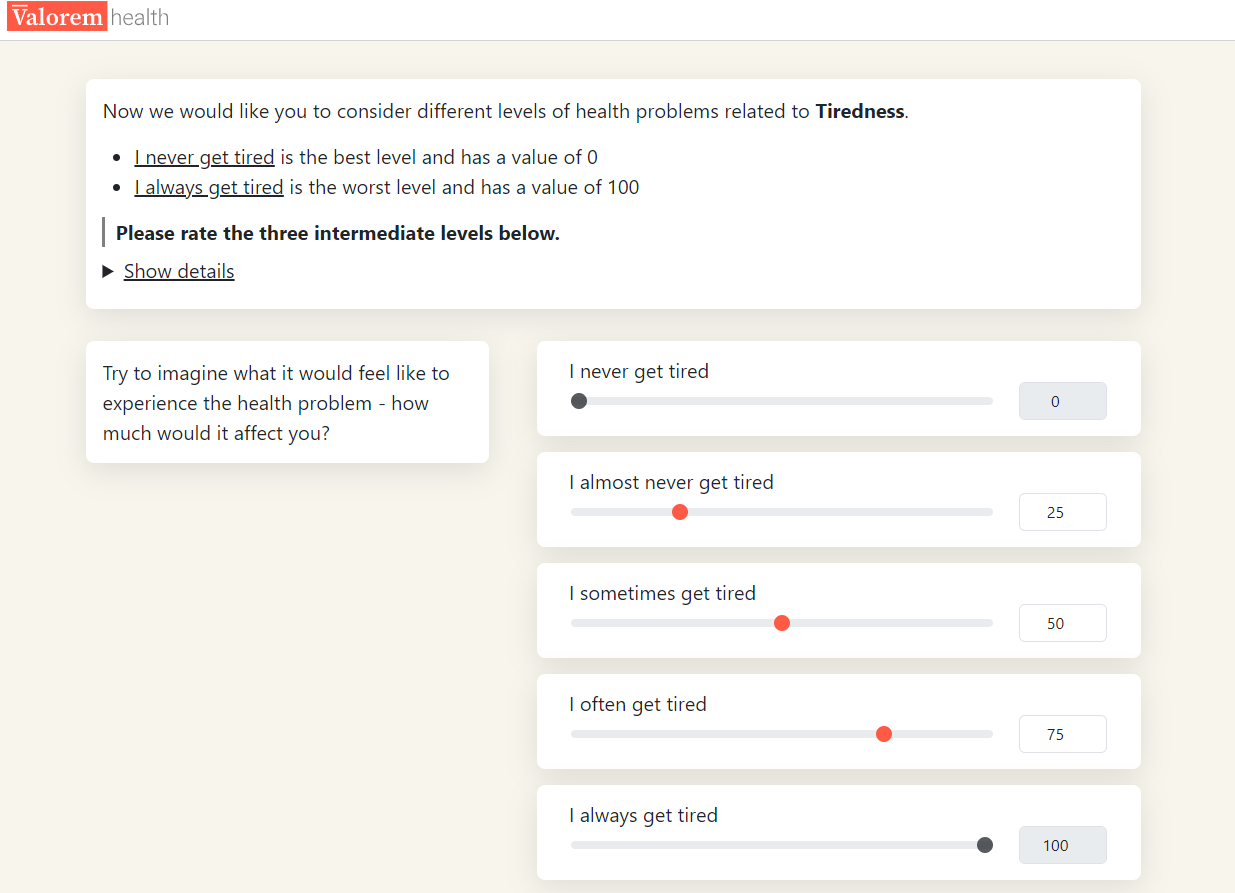
\includegraphics{../../outputs/figures/level_rating.png}

}

\subcaption{\label{fig-levelrating}Level rating: Tiredness}

\end{minipage}%
%
\begin{minipage}{0.50\linewidth}

\centering{

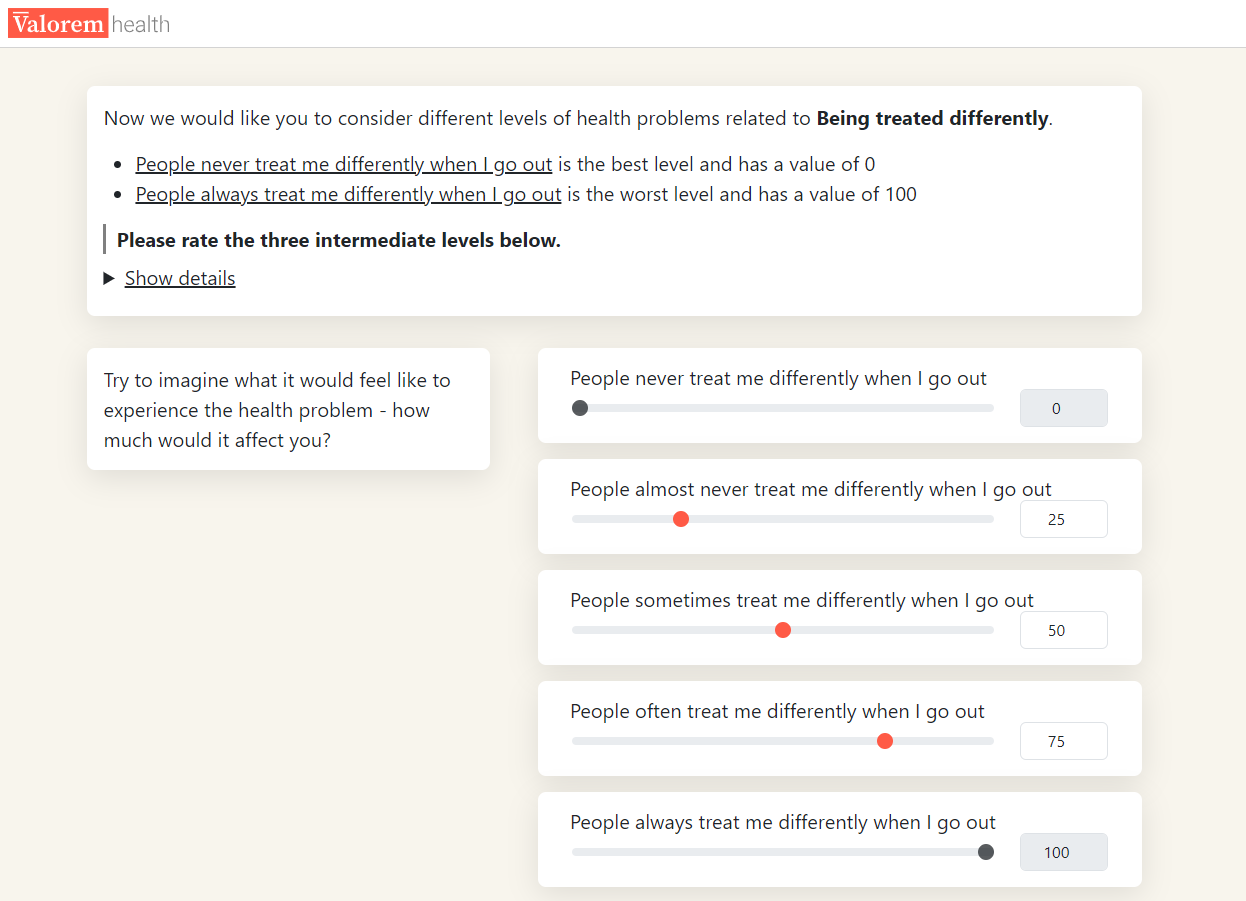
\includegraphics{../../outputs/figures/level_rating2.png}

}

\subcaption{\label{fig-levelrating2}Level rating: Treated differently}

\end{minipage}%

\caption{\label{fig-level}Level rating}

\end{figure}%

\subsubsection{Anchoring factor}\label{anchoring-factor}

A task is required to rescale the latent coefficients estimated via
combining level ratings and attribute weights onto the QALY scale.
Participants are presented with a binary choice between the PITS state
(or another state) of a given descriptive system and ``being dead''
(Figure~\ref{fig-anchor1}). If the PITS state is chosen, participants
are asked to rank the PITS state on a VAS from 1 (full health) to 0
(dead). If ``being dead'' is chosen, participants are asked to rank
``being dead'' on a VAS from 1 (full health) to 0 (PITS state)
(Figure~\ref{fig-anchor2}). Responses to these respective questions
provide the anchoring factor. Anchoring questions, such that PITS is
preferred to dead, are presented in Figure~\ref{fig-anchoring}.

\begin{figure}

\begin{minipage}{0.50\linewidth}

\centering{

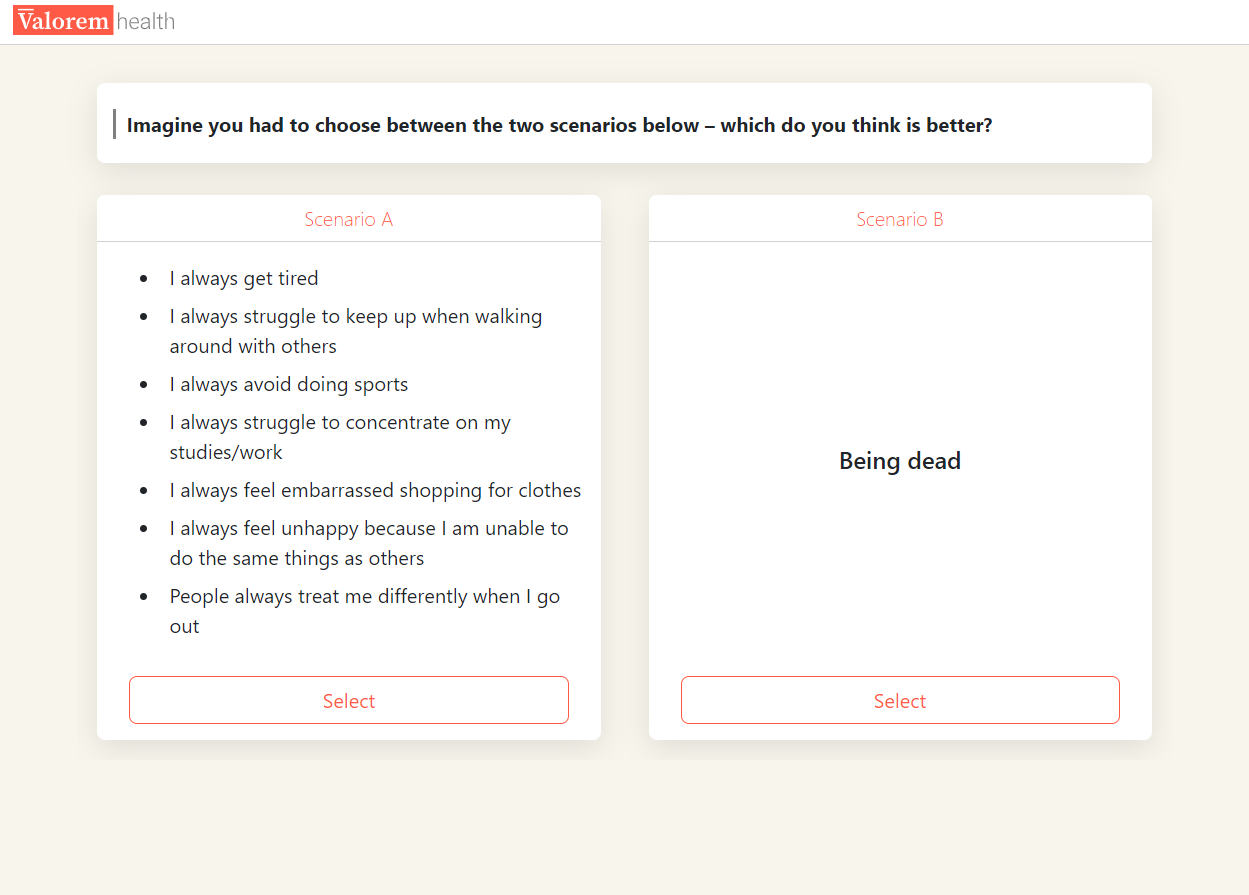
\includegraphics{../../outputs/figures/anchor1.png}

}

\subcaption{\label{fig-anchor1}PITS-dead}

\end{minipage}%
%
\begin{minipage}{0.50\linewidth}

\centering{

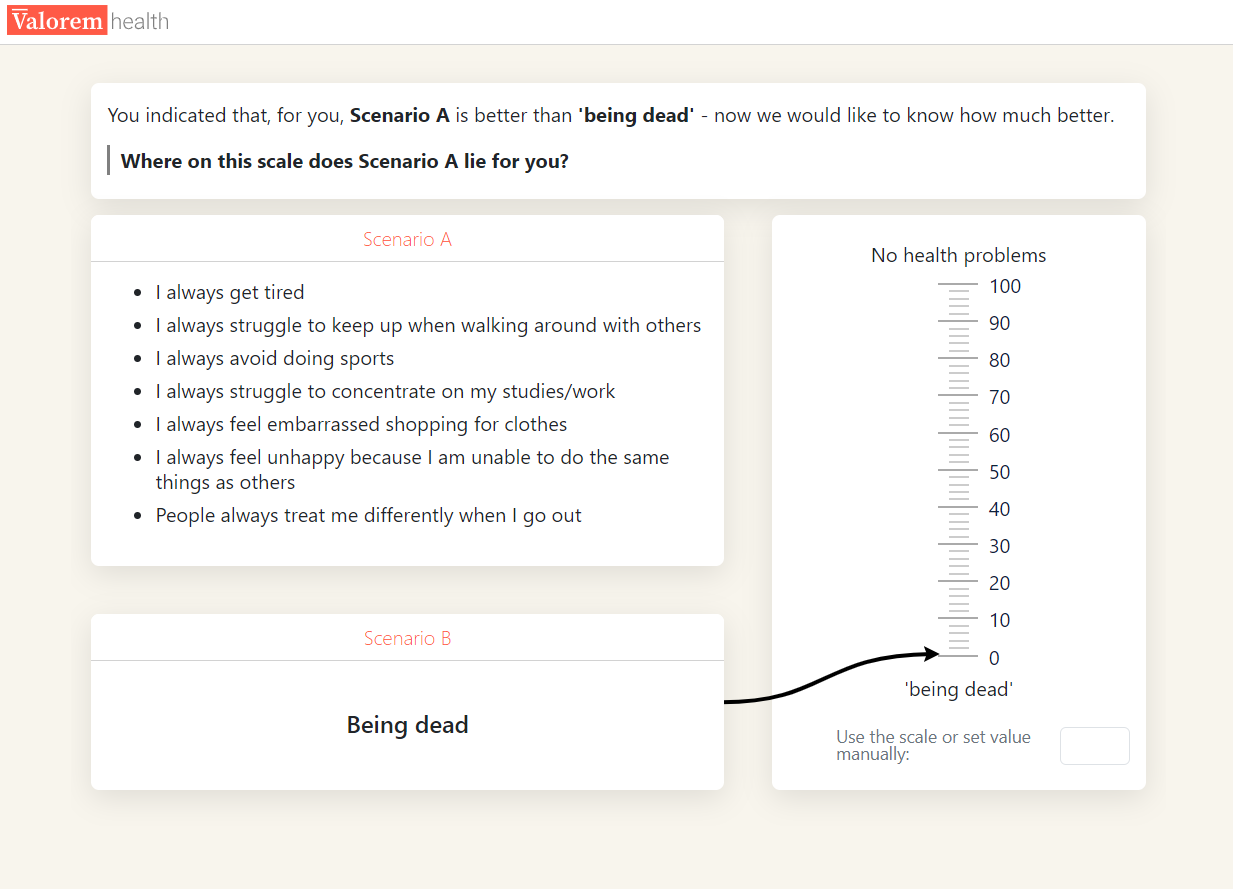
\includegraphics{../../outputs/figures/anchor2.png}

}

\subcaption{\label{fig-anchor2}PITS-VAS}

\end{minipage}%

\caption{\label{fig-anchoring}Anchoring factor}

\end{figure}%

\subsection{OPUF logic and mathematics}\label{sec-OPUF_methods}

This section presents the logic and underlying mathematics required to
convert the raw OPUF responses from one person into an anchored value
set for the WAItE descriptive system. This example assumes that level
ratings are obtained for each attribute separately, therefore
mathematics presented here differs to those presented elsewhere
\citep{Schneider2022TheStates}. Example response data are used for
demonstration in this section and are presented in
Table~\ref{tbl-exampledata}.

\subsubsection{Example responses}\label{example-responses}

\begin{longtable}[]{@{}
  >{\raggedright\arraybackslash}p{(\columnwidth - 14\tabcolsep) * \real{0.2812}}
  >{\raggedleft\arraybackslash}p{(\columnwidth - 14\tabcolsep) * \real{0.0625}}
  >{\raggedleft\arraybackslash}p{(\columnwidth - 14\tabcolsep) * \real{0.0833}}
  >{\raggedleft\arraybackslash}p{(\columnwidth - 14\tabcolsep) * \real{0.0729}}
  >{\raggedleft\arraybackslash}p{(\columnwidth - 14\tabcolsep) * \real{0.1458}}
  >{\raggedleft\arraybackslash}p{(\columnwidth - 14\tabcolsep) * \real{0.1458}}
  >{\raggedleft\arraybackslash}p{(\columnwidth - 14\tabcolsep) * \real{0.1250}}
  >{\raggedleft\arraybackslash}p{(\columnwidth - 14\tabcolsep) * \real{0.0833}}@{}}

\caption{\label{tbl-exampledata}Example individual responses to the
OPUF}

\tabularnewline

\toprule\noalign{}
\begin{minipage}[b]{\linewidth}\raggedright
Response
\end{minipage} & \begin{minipage}[b]{\linewidth}\raggedleft
Tired
\end{minipage} & \begin{minipage}[b]{\linewidth}\raggedleft
Walking
\end{minipage} & \begin{minipage}[b]{\linewidth}\raggedleft
Sports
\end{minipage} & \begin{minipage}[b]{\linewidth}\raggedleft
Concentration
\end{minipage} & \begin{minipage}[b]{\linewidth}\raggedleft
Embarrassment
\end{minipage} & \begin{minipage}[b]{\linewidth}\raggedleft
Unhappiness
\end{minipage} & \begin{minipage}[b]{\linewidth}\raggedleft
Treated
\end{minipage} \\
\midrule\noalign{}
\endhead
\bottomrule\noalign{}
\endlastfoot
Level rating: Never & 0 & 0 & 0 & 0 & 0 & 0 & 0 \\
Level rating: Almost Never & 14 & 26 & 21 & 15 & 16 & 12 & 19 \\
Level rating: Sometimes & 57 & 55 & 63 & 54 & 38 & 26 & 66 \\
Level rating: Often & 83 & 82 & 85 & 86 & 64 & 38 & 91 \\
Level rating: Always & 100 & 100 & 100 & 100 & 100 & 100 & 100 \\
Attribute Weighting & 28 & 33 & 36 & 45 & 100 & 34 & 56 \\

\end{longtable}

Level ratings (presented in Table~\ref{tbl-exampledata}) are converted
to coefficients bounded between 0-1 (shown in
Equation~\ref{eq-level-rescale}). Level rating coefficients are
presented in Equation~\ref{eq-level-matrix}. Attribute weights
(presented in Table~\ref{tbl-exampledata}) are then normalised to sum to
the value of 1 by dividing each weight by the sum of all weights (shown
in Equation~\ref{eq-weight-normalise}). Normalised attribute weights are
presented in Equation~\ref{eq-weight-vector}.

\begin{equation}\phantomsection\label{eq-level-rescale}{
    L_{ij} \cdot 0.01
}\end{equation}

\begin{equation}\phantomsection\label{eq-level-matrix}{
L_{ij} = 
\begin{bmatrix}
0 & 0 & 0 & 0 & 0 & 0 & 0 \\
0.14 & 0.26 & 0.21 & 0.15 & 0.16 & 0.12 & 0.19 \\
0.57 & 0.55 & 0.63 & 0.54 & 0.38 & 0.26 & 0.66 \\
0.83 & 0.82 & 0.85 & 0.86 & 0.64 & 0.38 & 0.91 \\
1 & 1 & 1 & 1 & 1 & 1 & 1 \\
\end{bmatrix}
}\end{equation}

\begin{equation}\phantomsection\label{eq-weight-normalise}{
    \frac{w_{j}}{\sum{w_j}}
}\end{equation}

\begin{equation}\phantomsection\label{eq-weight-vector}{
w_j = \begin{bmatrix}
    0.08& 0.10& 0.11& 0.14& 0.30& 0.10& 0.17
\end{bmatrix} 
}\end{equation}

Combining the attribute weights (Equation~\ref{eq-weight-vector}) with
the level coefficients (Equation~\ref{eq-level-matrix}) via element-wise
multiplication (shown in Equation~\ref{eq-element-wise-multiplication}
gives the coefficient matrix presented in
Equation~\ref{eq-coeff-matrix}. Once the coefficient matrix has been
estimated, preference values can be estimated on the 0-1 QALY scale
where the worst health state (PITS state denoted 5555555) is zero and
the best health state (denoted 1111111) is one. These latent
coefficients must now be rescaled to incorporate the results from the
PITS anchoring task so that the minimum utility value possible is equal
to the PITS value.

\begin{equation}\phantomsection\label{eq-element-wise-multiplication}{
    L_{ij} \cdot  w_{j} = {\tilde{M}}_{ij}
}\end{equation}

\begin{equation}\phantomsection\label{eq-coeff-matrix}{
\tilde{M}_{ij} =  
\begin{bmatrix}
0 & 0 & 0 & 0 & 0 & 0 & 0 \\
0.01 & 0.03 & 0.02 & 0.02 & 0.05 & 0.01 & 0.03 \\
0.05 & 0.05 & 0.07 & 0.07 & 0.11 & 0.03 & 0.11 \\
0.07 & 0.08 & 0.09 & 0.12 & 0.19 & 0.04 & 0.15 \\
0.08 & 0.10 & 0.11 & 0.14 & 0.30 & 0.10 & 0.17
\end{bmatrix}
}\end{equation}

To rescale the latent coefficient matrix to incorporate the anchoring
task, the coefficient matrix is multiplied by the compliment of the PITS
value (shown in Equation~\ref{eq-anchoring}) to give the anchored
coefficient matrix presented in Equation~\ref{eq-anchored-matrix}.

\begin{equation}\phantomsection\label{eq-anchoring}{
    \tilde{M}_{ij} \cdot (1-P) \quad \backepsilon \quad P = 0.2 
}\end{equation}

\begin{equation}\phantomsection\label{eq-anchored-matrix}{
\tilde{V}_{ij} =  
\begin{bmatrix}
0 & 0 & 0 & 0 & 0 & 0 & 0 \\
0.01 & 0.02 & 0.02 & 0.02 & 0.04 & 0.01 & 0.02 \\
0.04 & 0.04 & 0.06 & 0.06 & 0.09 & 0.02 & 0.09 \\
0.06 & 0.06 & 0.07 & 0.10 & 0.15 & 0.03 & 0.12 \\
0.06 & 0.08 & 0.09 & 0.11 & 0.24 & 0.08 & 0.14 \\
\end{bmatrix}
}\end{equation}

Once the attribute and level labels are reintroduced to the anchored
coefficient matrix this forms the value set which presents the
disutility corresponding to each attribute level combination presented
in the WAItE. Table~\ref{tbl-example-valueset} presents the WAItE
example PUF value set. Equation~\ref{eq-HS123} present examples of how
to estimate a utility value given a specific WAItE health state.

\begin{longtable}[]{@{}
  >{\raggedright\arraybackslash}p{(\columnwidth - 14\tabcolsep) * \real{0.1649}}
  >{\raggedleft\arraybackslash}p{(\columnwidth - 14\tabcolsep) * \real{0.0619}}
  >{\raggedleft\arraybackslash}p{(\columnwidth - 14\tabcolsep) * \real{0.0825}}
  >{\raggedleft\arraybackslash}p{(\columnwidth - 14\tabcolsep) * \real{0.0722}}
  >{\raggedleft\arraybackslash}p{(\columnwidth - 14\tabcolsep) * \real{0.1443}}
  >{\raggedleft\arraybackslash}p{(\columnwidth - 14\tabcolsep) * \real{0.1443}}
  >{\raggedleft\arraybackslash}p{(\columnwidth - 14\tabcolsep) * \real{0.1237}}
  >{\raggedleft\arraybackslash}p{(\columnwidth - 14\tabcolsep) * \real{0.2062}}@{}}

\caption{\label{tbl-example-valueset}WAItE example PUF value set}

\tabularnewline

\toprule\noalign{}
\begin{minipage}[b]{\linewidth}\raggedright
Attribute level
\end{minipage} & \begin{minipage}[b]{\linewidth}\raggedleft
Tired
\end{minipage} & \begin{minipage}[b]{\linewidth}\raggedleft
Walking
\end{minipage} & \begin{minipage}[b]{\linewidth}\raggedleft
Sports
\end{minipage} & \begin{minipage}[b]{\linewidth}\raggedleft
Concentration
\end{minipage} & \begin{minipage}[b]{\linewidth}\raggedleft
Embarrassment
\end{minipage} & \begin{minipage}[b]{\linewidth}\raggedleft
Unhappiness
\end{minipage} & \begin{minipage}[b]{\linewidth}\raggedleft
Treated differently
\end{minipage} \\
\midrule\noalign{}
\endhead
\bottomrule\noalign{}
\endlastfoot
Never & 0.00 & 0.00 & 0.00 & 0.00 & 0.00 & 0.00 & 0.00 \\
Almost Never & 0.01 & 0.02 & 0.02 & 0.02 & 0.04 & 0.01 & 0.02 \\
Sometimes & 0.04 & 0.04 & 0.06 & 0.06 & 0.09 & 0.02 & 0.09 \\
Often & 0.06 & 0.06 & 0.07 & 0.10 & 0.15 & 0.03 & 0.12 \\
Always & 0.06 & 0.08 & 0.09 & 0.11 & 0.24 & 0.08 & 0.14 \\

\end{longtable}

\begin{equation}\phantomsection\label{eq-HS123}{
\begin{aligned}
\text{Health State [5555555]} & \Rightarrow 1 - (0.06 + 0.08 + 0.09 + 0.11 + 0.24 + 0.08 + 0.14) = 0.20 \\
\text{Health State [5223445]} & \Rightarrow 1 - (0.06 + 0.02 + 0.02 + 0.06 + 0.15 + 0.03 + 0.14) = 0.52 \\
\text{Health State [2222222]} & \Rightarrow 1 - (0.03 + 0.02 + 0.01 + 0.01 + 0.02 + 0.02 + 0.04) = 0.85
\end{aligned}
}\end{equation}

\subsection{Aggregation to social utility
function}\label{aggregation-to-social-utility-function}

The OPUF is designed to be able to estimate personal utility functions
and so estimation occurs on an individual basis. Aggregating personal
utility functions to a social utility function (SUF) takes place by
taking a mean of all the individual personal utility functions from your
sample. This operation is presented in Equation~\ref{eq-meanvalueset}.

\begin{equation}\phantomsection\label{eq-meanvalueset}{
\bar{V}_{{ij}} = \frac{\sum_{\tilde{V}_{{ij}}}^{}}{N}
}\end{equation}

\section{Methods}\label{methods}

\subsection{Recruitment}\label{recruitment}

This study recruited (n=300) adults to respond to a quality-of-life
survey hosted online. Study participants were recruited based on
specific quotas to form a representative sample based on UK census data.
The survey was hosted on the \href{https://www.prolific.com}{Prolific}
platform which invited paid respondents to complete the Weight-specific
Adolescent Instrument for Economic evaluation (WAItE) version of the
Online Personal Utility Functions (OPUF) survey. A demonstration of the
OPUF survey and questions is available
\href{https://survey.valorem.health/waite_opuf_adult2}{here}. Informed
consent was obtained at the outset of the survey and participants
reserved the right to withdraw at any point without giving a reason.
Participants who withdrew were not paid and their data deleted.
Participation in this survey was estimated to take approximately fifteen
minutes to complete and participants received £2.50 as a payment upon
completion. This is in line with reimbursements rates from other OPUF
studies \citep{Schneider2022TheStates, Bray2024DevelopmentImpairment}
and is in line with recommended reimbursement rates from
\href{https://www.prolific.com}{Prolific}. The survey was designed to be
an unassisted survey administered online (no face-to-face contact) and
no identifiable data was collected. Statistical analysis was conducted
on the survey data. Newcastle University Medical School Ethics Committee
approved this study (reference 49737/2023). The survey structure is
detailed in Section~\ref{sec-surveystructure}.

\subsection{Survey structure}\label{sec-surveystructure}

\begin{enumerate}
\def\labelenumi{\arabic{enumi}.}
\tightlist
\item
  Consent and Prolific ID: Participants were asked to consent to
  participate and enter their unique Prolific ID. This enables
  demographic information held by Prolific on their participants to be
  linked to each respondent.
\item
  WAItE descriptive system: Participants were asked to complete the
  WAItE descriptive system (presented in
  Figure~\ref{fig-waite-descriptive})to describe their current health
  state.
\item
  Dimension selection: Participants were presented with the worst level
  for each WAItE dimension and asked to choose which health problem
  would have the most negative impact on their quality of life. The
  dimension chosen is then used in the subsequent dimension swing
  weighting task.\\
\item
  Dimension swing weighting: Participants were presented with each
  dimension in the WAItE and asked to consider an improvement from the
  worst level of that dimension to the best level of that dimension.
  Participants were asked to rank this improvement on a visual slider
  from 0-100 where the most important dimension (chosen in the previous
  task) is fixed at 100. Participants were reminded to use their most
  important dimension as a reference point.\\
\item
  Level rating: Participants were presented with a specific dimension of
  the WAItE and shown each level within that dimension. Levels best and
  worst (never and always) were fixed at 0 and 100 respectively.
  Participants were asked to rank the intermediate levels within each
  dimension using the fixed levels as a reference point.
\item
  Anchoring: Participants were presented with a binary choice asking
  whether they prefer the worst state of the WAItE (PITS state) or
  death. If participants choose the worst state of the WAItE, a second
  question is asked which asks them to rank the WAITE PITS state on a
  visual analogue scale where zero is labelled as being dead and one
  hundred is labelled as no health problems. If participants choose
  death in the binary choice, they were asked to rank being dead on a
  visual analogue scale where zero is labelled as the WAItE PITS state
  and one hundred is labelled as no health problems.
\item
  Survey feedback and demographic questions: Participants were asked
  about how difficult they found the task to complete and demographic
  information on age, gender, ethnicity, education, employment and
  weight status.
\end{enumerate}

\begin{figure}

\centering{

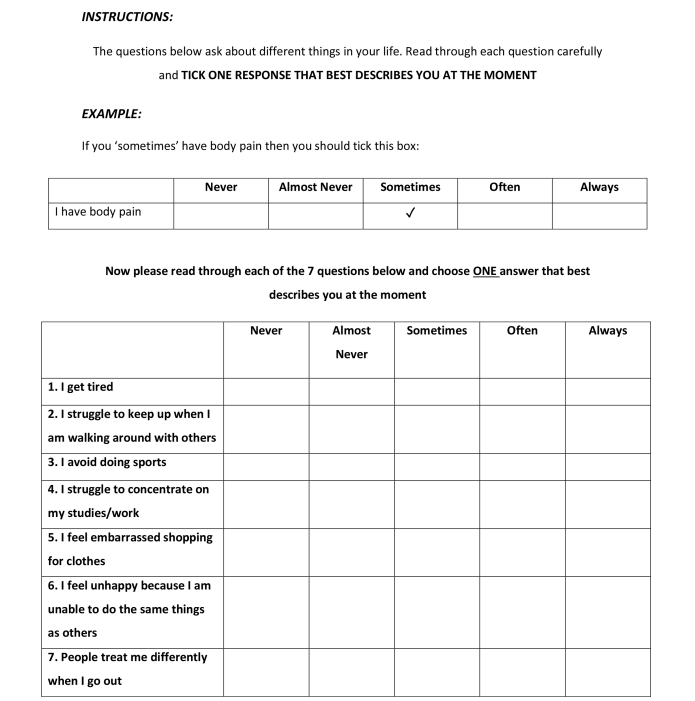
\includegraphics{../../outputs/figures/WAItE descriptive.png}

}

\caption{\label{fig-waite-descriptive}WAItE descriptive system}

\end{figure}%

\subsection{Missing data}\label{missing-data}

Through the survey design process the potential for large amounts of
missing data has been mitigated by ensuring responses were compulsory to
certain questions. However for ethical reasons, we allowed participants
to not answer the questions relating to death. For participants who do
not provide responses to the anchoring questions, their responses were
imputed using multiple imputation by chained equations (MICE)
\citep{White2011MultiplePractice} which were informed by demographic
information and dimension weighting responses.

\subsection{Preference heterogeneity}\label{preference-heterogeneity}

As personal utility function are estimated on an individual basis,
exploring preference heterogeneity between individuals in the sample is
straightforward. Investigating the heterogeneity of preferences between
individuals, requires a measure of dis/similarity to quantify how far
apart two PUFs are \citep{Schneider2024ExploringLevel}. The measurement
and estimation of preference heterogeneity in this section will follow
methods detailed by Schneider et al.~(2024)
\citep{Schneider2024ExploringLevel}. Each PUF estimated in this study
was represented by a vector of 78,125 health state utility values for
each respondent in the sample. In order to assess the dis/similarity
between these PUFs, we used the euclidean difference measure (EUD).
Analogous to a line between two points on a two dimensional plane, the
EUD between two PUFs denotes the shortest path length in a 78,125
dimensional space. It is computed as the square root of the sum of the
squared differences between the PUFs of individuals \(i\) and \(j\)
(presented in Equation~\ref{eq-EUD}). Once PUFs have been estimated for
all individuals in the sample, pairwise EUD was estimated for all
possible pairwise combinations within the sample. Pairwise EUD was
stored in an {[}N \(\times\) N{]} distance matrix.

\begin{equation}\phantomsection\label{eq-EUD}{ 
  \begin{aligned}
    d_{EUD}(i,j) & =\sqrt{\sum_{}^{}(u_{i}(s_{1})-u_{j}(s_{1}))^{2}+ ... +(u_{i}(s_{78125})-u_{j}(s_{78125}))^{2}}\\
      & \backepsilon \quad \quad s = \{1111111, 2111111, ..., 5555555\}\\
  \end{aligned}
}\end{equation}

\subsection{Permutational analysis of
variance}\label{permutational-analysis-of-variance}

Permutational analysis of variance (PERMANOVA), analogous to analysis of
variance, is a geometric partitioning of variation across a multivariate
data cloud, definied in the space of any given dissimilarity measure, in
response to one or more groups
\citep{Anderson2017, Anderson2013PERMANOVATesting}. This method of
statistical testing has been used most commonly in ecological research
to test for population dispersion among different subgroups
\citep{Souza2013PopulationEstuary}. PERMANOVA decomposes the total
distances between observations (SS\(_T\)) into within-groups (SS\(_W\))
and between groups sum-of-squares (SS\(_B\)).
Equation~\ref{eq-sumsquares} details the estimation of total and
within-groups sum-of-squares. Mathematical notation presented here is
reproduced from Schneider et al.~(2024)
\citep{Schneider2024ExploringLevel} for consistency.

\begin{equation}\phantomsection\label{eq-sumsquares}{ 
    SS_{T} = \frac{1}{N}\sum_{i=1}^{N-1}\sum_{j=i+1}^{N}d(i,j)^{2}; \quad SS_{W} = \sum_{i=1}^{N-1}\sum_{j=i+1}^{N}d(i,j)^{2}\epsilon_{ij}^{\ell}/n_{\ell}
}\end{equation}

where N is the total sample size (=300), \(d(i,j)^2\) is the squared
distance between the PUFs of participants \(i\) and \(j\),
\(\epsilon_{i,j}\) indicator which is 1, if participants \(i\) and \(j\)
belong to the same group, and 0 if they do not, and \(n_{\ell}\) is the
size for group \(\ell\). Then, SS\(_B\) can then be calculated as
SS\(_B\) = SS\(_T\) -- SS\(_W\), which allows calculating the pseudo F
statistic for \(p\) groups:

\begin{equation}\phantomsection\label{eq-ssb}{
F= \frac{(\frac{SS_B}{p-1})}{(\frac{SS_W}{N-p})}
}\end{equation}

Further details about the mathematical and statistical properties of
PERMANOVA are available elsewhere
\citep{Schneider2024ExploringLevel, Anderson2017, Anderson2013PERMANOVATesting}.
In this study, we used PERMANOVA to explore the variability in WAItE
health state preferences (individual value sets) between various
subgroups. A multivariate PERMANOVA model was estimated with subgroups
of: age, gender, self-reported weight status, education, employment
status and ethncity.

\subsection{Sensitivity analysis}\label{sensitivity-analysis}

In an experimental sensitivity analysis, preference heterogeneity was
assessed using EUD estimated based on individual's personal utility
functions anchored using the social PITS utility value (henceforth
referred to as EUD2). This differed to prior preference heterogeneity
estimation as individual variation in PITS utility values were not
included in the EUD2 estimation. EUD2 was entirely composed by
differences in level ratings and attribute weights. Further details on
the derivation of EUD2 are presented in Section~\ref{sec-appendix1}.

\section{Results}\label{results}

\subsection{Study participants}\label{study-participants}

A sample of 334 individuals were approached to participate in the study
via the survey company \href{https://www.prolific.com}{Prolific}.
Individuals that successfully inputted their unique Prolific ID and
obtained a correct completion code from the end of the study were
included in the analysis sample and received a small payment (£2.50) for
their participation. Seven participants were excluded from the study as
they had an incorrect completion code and did not enter the correct
unique Prolific ID. Therefore no data was available on those seven
participants and so they were excluded from the analysis. An additional
participant was excluded from the analysis due to completing the survey
in eighteen seconds (well under the prespecified minimum time limit of 2
minutes). Two respondents timed-out while completing the survey and were
therefore not included. Twenty-four individuals chose not complete the
study (referred to by Prolific as `returned' participants). This left an
analysis sample of N=300 participants who successfully completed the
survey. A representative sample based on UK census data was obtained
from Prolific. A summary of demographic information collected in the
OPUF are presented in Table~\ref{tbl-demographic}.

\subsection{Survey duration}\label{survey-duration}

The mean (SD) and median (IQR) survey completion time in minutes was
9.66 (5.85) and 8.15 (5.88; 11.89). Table~\ref{tbl-time} summarises how
much time was spent completing each individual section of the survey.

\begin{longtable}[]{@{}
  >{\raggedright\arraybackslash}p{(\columnwidth - 8\tabcolsep) * \real{0.2941}}
  >{\raggedright\arraybackslash}p{(\columnwidth - 8\tabcolsep) * \real{0.2059}}
  >{\raggedright\arraybackslash}p{(\columnwidth - 8\tabcolsep) * \real{0.3088}}
  >{\raggedright\arraybackslash}p{(\columnwidth - 8\tabcolsep) * \real{0.0882}}
  >{\raggedright\arraybackslash}p{(\columnwidth - 8\tabcolsep) * \real{0.1029}}@{}}

\caption{\label{tbl-time}Survey completion times (secs)}

\tabularnewline

\toprule\noalign{}
\begin{minipage}[b]{\linewidth}\raggedright
Section
\end{minipage} & \begin{minipage}[b]{\linewidth}\raggedright
Mean (SD)
\end{minipage} & \begin{minipage}[b]{\linewidth}\raggedright
Median (Q1; Q3)
\end{minipage} & \begin{minipage}[b]{\linewidth}\raggedright
Min
\end{minipage} & \begin{minipage}[b]{\linewidth}\raggedright
Max
\end{minipage} \\
\midrule\noalign{}
\endhead
\bottomrule\noalign{}
\endlastfoot
WAItE & 73 (90.1) & 53 (38; 77) & 10 & 1066 \\
Dimension ranking & 35.4 (50.6) & 26 (16; 40) & 2 & 741 \\
Dimension weighting & 115.7 (94.9) & 91.5 (69.8; 142.2) & 18 & 1380 \\
Level rating & 220.5 (206.4) & 171 (119; 249) & 34 & 2158 \\
PITS vs death & 25.5 (45.4) & 16.5 (11; 25.2) & 4 & 620 \\
PITS-VAS & 37.3 (39.2) & 29 (21; 45) & 5 & 605 \\
PITS-VAS & 37.3 (39.2) & 29 (21; 45) & 5 & 605 \\
Total (secs) & 579.5 (351.1) & 489.2 (352.5; 713.4) & 126.7 & 3738.2 \\
Total (mins) & 9.66 (5.85) & 8.15 (5.88; 11.89) & 2.11 & 62.3 \\

\end{longtable}

\subsection{WAItE descriptive system}\label{waite-descriptive-system}

Responses to the WAItE descriptive system are presented in Table
\citep{tab-demographic}. Feeling tired and avoiding doing sport were the
attributes that were most frequently experienced by participants in our
analysis sample. WAItE summary statistics were in line with results from
previous studies \citep{Robinson2019EstimatingEvaluation}.

\begin{longtable}[]{@{}ll@{}}

\caption{\label{tbl-demographic}Summary of demographic information
collected in the OPUF}

\tabularnewline

\toprule\noalign{}
Participant Characteristics (N=300) & N (\%) \\
\midrule\noalign{}
\endhead
\bottomrule\noalign{}
\endlastfoot
Age & \\
18-24 & 32 (10.9\%) \\
25-34 & 50 (17\%) \\
35-44 & 48 (16.3\%) \\
45-54 & 49 (16.7\%) \\
55-64 & 81 (27.6\%) \\
65-90 & 34 (11.6\%) \\
Not Stated & 6 (2.0\%) \\
Gender & \\
Female & 154 (51\%) \\
Male & 144 (48\%) \\
Non-binary & 1 (0\%) \\
Ethnicity & \\
White & 251 (84\%) \\
Asian & 23 (8\%) \\
Black & 11 (4\%) \\
Mixed & 10 (3\%) \\
Other & 5 (2\%) \\
Weight Status & \\
Normal & 154 (51\%) \\
Overweight & 104 (35\%) \\
Obese & 30 (10\%) \\
Underweight & 8 (3\%) \\
Prefer not to say & 4 (1\%) \\
Education & \\
Degree & 147 (49\%) \\
A Level & 64 (21\%) \\
Higher Education & 46 (15\%) \\
Other & 20 (7\%) \\
GCSE A-C & 18 (6\%) \\
GCSE D-G & 5 (2\%) \\
Occupation & \\
Full-time & 130 (43\%) \\
Part-time & 62 (21\%) \\
Not Paid & 30 (10\%) \\
Other & 31 (10\%) \\
Student & 17 (6\%) \\
Unemployed & 18 (6\%) \\
Not Stated & 9 (3\%) \\
Starting a New Job & 3 (1\%) \\
WAItE & Mean (SD) \\
Tiredness & 3.4 (0.8) \\
Walking & 2.1 (1.1) \\
Sport & 3.3 (1.3) \\
Concentration & 2.7 (1.0) \\
Embarrassment & 2.2 (1.2) \\
Unhappiness & 2.3 (1.0) \\
Treated differently & 1.9 (0.9) \\
Total & 17.8 (4.8) \\

\end{longtable}

\subsection{Level ratings}\label{level-ratings-1}

Level ratings are presented individually for each different attribute in
Table~\ref{tbl-level}. The best and worst levels (\textit{Always} and
\textit{Never}) were fixed at 0 and 100 respectively. The second best
level (\textit{Almost never}) had the lowest VAS score in the Sports and
Embarrassment attribute, while the second worst level (\textit{Often})
had the highest VAS score in the Concentration attribute. In this
question, higher VAS scores indicate worse states of health.

\begin{longtable}[]{@{}
  >{\raggedright\arraybackslash}p{(\columnwidth - 8\tabcolsep) * \real{0.3580}}
  >{\raggedright\arraybackslash}p{(\columnwidth - 8\tabcolsep) * \real{0.1975}}
  >{\raggedright\arraybackslash}p{(\columnwidth - 8\tabcolsep) * \real{0.1975}}
  >{\raggedright\arraybackslash}p{(\columnwidth - 8\tabcolsep) * \real{0.1235}}
  >{\raggedright\arraybackslash}p{(\columnwidth - 8\tabcolsep) * \real{0.1235}}@{}}

\caption{\label{tbl-level}Summary of OPUF level ratings by attribute}

\tabularnewline

\toprule\noalign{}
\begin{minipage}[b]{\linewidth}\raggedright
Section
\end{minipage} & \begin{minipage}[b]{\linewidth}\raggedright
Mean (SD)
\end{minipage} & \begin{minipage}[b]{\linewidth}\raggedright
Median (Q1; Q3)
\end{minipage} & \begin{minipage}[b]{\linewidth}\raggedright
Min
\end{minipage} & \begin{minipage}[b]{\linewidth}\raggedright
Max
\end{minipage} \\
\midrule\noalign{}
\endhead
\bottomrule\noalign{}
\endlastfoot
\textbf{Tired} & \textbf{} & \textbf{} & \textbf{} & \textbf{} \\
Almost never & 20.323 (23.208) & 10 (5; 25) & 0 & 100 \\
Sometimes & 36.31 (19.185) & 33.5 (20; 50) & 0 & 100 \\
Often & 62.217 (23.934) & 70 (50; 80) & 0 & 100 \\
\textbf{Walking} & \textbf{} & \textbf{} & \textbf{} & \textbf{} \\
Almost never & 19.39 (21.839) & 10 (6; 21) & 0 & 100 \\
Sometimes & 37.677 (19.373) & 40 (24; 50) & 0 & 100 \\
Often & 62.967 (26.167) & 71 (50; 80) & 0 & 100 \\
\textbf{Sports} & \textbf{} & \textbf{} & \textbf{} & \textbf{} \\
Almost never & 16.63 (20.978) & 10 (5; 20) & 0 & 100 \\
Sometimes & 29.487 (22.015) & 25 (10; 45) & 0 & 100 \\
Often & 49.843 (29.624) & 50.5 (24.5; 75) & 0 & 100 \\
\textbf{Concentration} & \textbf{} & \textbf{} & \textbf{} &
\textbf{} \\
Almost never & 21.393 (22.1) & 14 (7; 25) & 0 & 100 \\
Sometimes & 41.56 (20.101) & 40 (25.8; 53.2) & 0 & 100 \\
Often & 64.503 (26.195) & 73 (50; 80.2) & 0 & 100 \\
\textbf{Embarrassment} & \textbf{} & \textbf{} & \textbf{} &
\textbf{} \\
Almost never & 16.59 (22.292) & 10 (4; 20) & 0 & 100 \\
Sometimes & 29.417 (21.615) & 25 (10; 50) & 0 & 100 \\
Often & 47.91 (30.445) & 50 (20; 75) & 0 & 100 \\
\textbf{Unhappiness} & \textbf{} & \textbf{} & \textbf{} & \textbf{} \\
Almost never & 21.13 (22.235) & 13 (6; 25) & 0 & 100 \\
Sometimes & 41.363 (22.128) & 41.5 (25; 56) & 0 & 100 \\
Often & 63.557 (28.187) & 75 (50; 85) & 0 & 100 \\
\textbf{Treated differently} & \textbf{} & \textbf{} & \textbf{} &
\textbf{} \\
Almost never & 20.93 (24.366) & 11 (5; 25) & 0 & 100 \\
Sometimes & 35.52 (22.774) & 34.5 (19.8; 50) & 0 & 100 \\
Often & 55.857 (30.552) & 60.5 (31; 80) & 0 & 100 \\

\end{longtable}

\subsection{Attribute weights}\label{attribute-weights}

Summary statistics of attribute weightings are presented in
Table~\ref{tbl-attribute}. On average, Tiredness (76.5) and Unhappiness
(70) were considered to be more important to participants than
Embarrassment (40.1) and Sports (42.3). There was less variability in
attribute weighting responses to Tiredness than responses to Treated
differently or Embarrassment. Figure~\ref{fig-rai} illustrates the
relative attribute importance (RAI) among WAItE attributes.

\begin{longtable}[]{@{}
  >{\raggedright\arraybackslash}p{(\columnwidth - 8\tabcolsep) * \real{0.3077}}
  >{\raggedright\arraybackslash}p{(\columnwidth - 8\tabcolsep) * \real{0.2051}}
  >{\raggedright\arraybackslash}p{(\columnwidth - 8\tabcolsep) * \real{0.2308}}
  >{\raggedright\arraybackslash}p{(\columnwidth - 8\tabcolsep) * \real{0.1282}}
  >{\raggedright\arraybackslash}p{(\columnwidth - 8\tabcolsep) * \real{0.1282}}@{}}

\caption{\label{tbl-attribute}Summary of OPUF attribute weights and
anchoring responses}

\tabularnewline

\toprule\noalign{}
\begin{minipage}[b]{\linewidth}\raggedright
Section
\end{minipage} & \begin{minipage}[b]{\linewidth}\raggedright
Mean (SD)
\end{minipage} & \begin{minipage}[b]{\linewidth}\raggedright
Median (Q1; Q3)
\end{minipage} & \begin{minipage}[b]{\linewidth}\raggedright
Min
\end{minipage} & \begin{minipage}[b]{\linewidth}\raggedright
Max
\end{minipage} \\
\midrule\noalign{}
\endhead
\bottomrule\noalign{}
\endlastfoot
Tired & 76.513 (28.358) & 90 (60; 100) & 1 & 100 \\
Walking & 65.53 (32.49) & 75 (40; 100) & 0 & 100 \\
Sports & 42.32 (32.81) & 35 (11; 70) & 0 & 100 \\
Concentration & 67.897 (30.949) & 80 (44; 99.2) & 0 & 100 \\
Embarrassment & 40.143 (34.344) & 30 (9; 70) & 0 & 100 \\
Unhappiness & 69.997 (31.946) & 80 (50; 100) & 0 & 100 \\
Treated differently & 52.093 (35.564) & 50 (15.8; 86) & 0 & 100 \\
\textbf{Anchoring} & \textbf{} & \textbf{} & \textbf{} & \textbf{} \\
PITS preferred to death & 0.879 (0.327) & 1 (1; 1) & 0 & 1 \\
PITS-VAS & 56.057 (31.287) & 54 (30; 85) & 0 & 100 \\
Dead-VAS & 42.528 (31.583) & 38.5 (13.2; 63.5) & 1 & 100 \\
PITS VAS uncensored & -0.025 (5.95) & 0.5 (0.2; 0.8) & -99 & 1 \\
PITS VAS censored & 0.431 (0.485) & 0.5 (0.2; 0.8) & -1 & 1 \\
PITS Utility Value & 0.282 (1.456) & 0.5 (0.2; 0.8) & -14.3 & 1 \\

\end{longtable}

\begin{figure}

\centering{

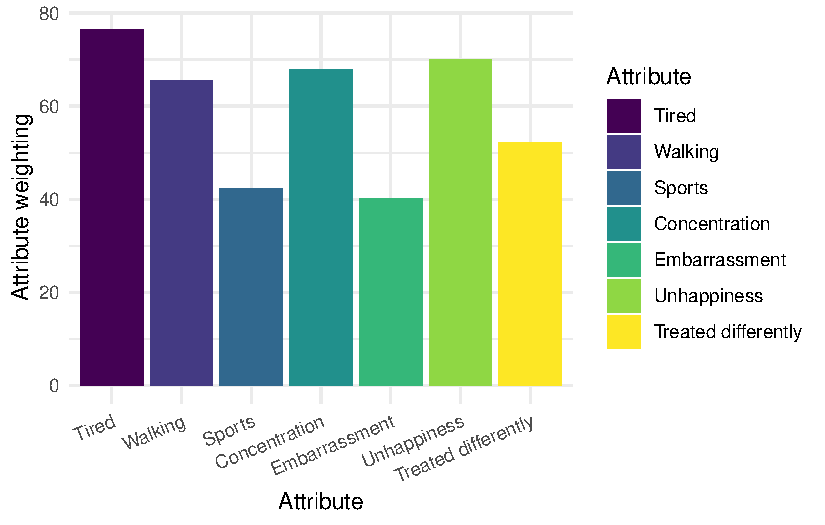
\includegraphics{quarto_files/figure-pdf/fig-rai-1.pdf}

}

\caption{\label{fig-rai}Relative attribute importance}

\end{figure}%

\subsection{Anchoring}\label{anchoring}

The majority of respondents in the sample preferred the WAItE PITS state
to being dead (87\%). Therefore, 13\% of participants answered the
dead-VAS and 87\% answered the PITS-VAS. A proportion of participants
did not answer the anchoring task (1.67\%). After winsorizing extreme
values (top and bottom 0.1\%) \citep{2003ApplyingTechniques} and
conducting multiple imputation by chained equations on the missing
values, the mean (SD) and median (IQR) PITS utility value was 0.282
(1.456) and 0.5 (0.6). The distribution of WAItE PITS utility values
(after winsorizing and imputation) is presented in
Figure~\ref{fig-hist}.

\begin{figure}

\centering{

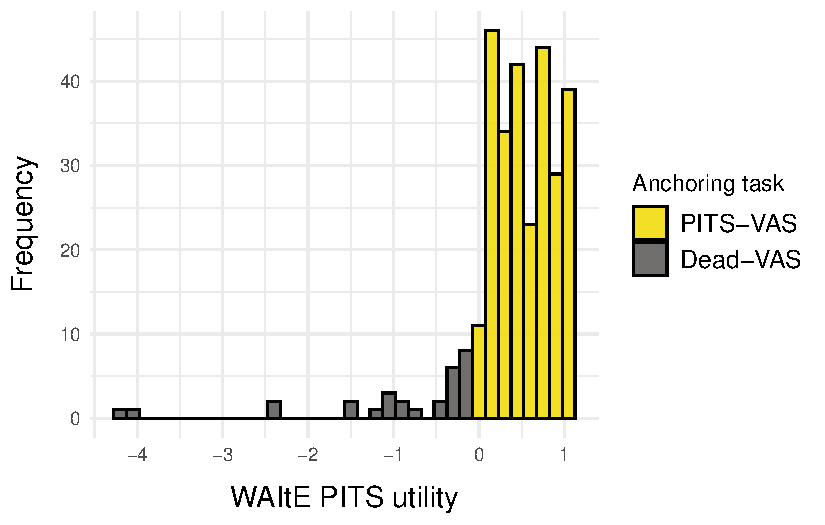
\includegraphics{quarto_files/figure-pdf/fig-hist-1.pdf}

}

\caption{\label{fig-hist}Distribution of PITS utility values}

\end{figure}%

\subsection{Social utility function
estimation}\label{social-utility-function-estimation}

Personal utility functions were estimated individually for each
participant in our analysis sample via methods outlined in
Section~\ref{sec-OPUF_methods}. After this, individual PUFs were
aggregated into a group utility function and anchored using the group
PITS utility value (0.282) to give the social utility function.
Descriptive statistics from the social utility function are presented in
Table~\ref{tbl-suf} whereby the mean values can be used to estimate
utility values for WAItE health states.

\begin{longtable}[]{@{}
  >{\raggedright\arraybackslash}p{(\columnwidth - 8\tabcolsep) * \real{0.3187}}
  >{\raggedright\arraybackslash}p{(\columnwidth - 8\tabcolsep) * \real{0.2308}}
  >{\raggedright\arraybackslash}p{(\columnwidth - 8\tabcolsep) * \real{0.2308}}
  >{\raggedright\arraybackslash}p{(\columnwidth - 8\tabcolsep) * \real{0.1099}}
  >{\raggedright\arraybackslash}p{(\columnwidth - 8\tabcolsep) * \real{0.1099}}@{}}

\caption{\label{tbl-suf}Social utility function based on 300 PUFs}

\tabularnewline

\toprule\noalign{}
\begin{minipage}[b]{\linewidth}\raggedright
Dimension Level
\end{minipage} & \begin{minipage}[b]{\linewidth}\raggedright
Mean (95\% CI)
\end{minipage} & \begin{minipage}[b]{\linewidth}\raggedright
Median (Q1; Q3)
\end{minipage} & \begin{minipage}[b]{\linewidth}\raggedright
Min
\end{minipage} & \begin{minipage}[b]{\linewidth}\raggedright
Max
\end{minipage} \\
\midrule\noalign{}
\endhead
\bottomrule\noalign{}
\endlastfoot
\textbf{Tired} & \textbf{} & \textbf{} & \textbf{} & \textbf{} \\
Almost never & 0.029 (0.025; 0.033) & 0.016 (0.007; 0.033) & 0 &
0.279 \\
Sometimes & 0.052 (0.048; 0.057) & 0.043 (0.024; 0.07) & 0 & 0.311 \\
Often & 0.088 (0.082; 0.094) & 0.086 (0.052; 0.112) & 0 & 0.359 \\
Always & 0.14 (0.133; 0.148) & 0.126 (0.101; 0.161) & 0.006 & 0.479 \\
\textbf{Walking} & \textbf{} & \textbf{} & \textbf{} & \textbf{} \\
Almost never & 0.021 (0.018; 0.024) & 0.013 (0.006; 0.026) & 0 &
0.179 \\
Sometimes & 0.045 (0.041; 0.049) & 0.04 (0.019; 0.062) & 0 & 0.192 \\
Often & 0.075 (0.069; 0.082) & 0.074 (0.028; 0.102) & 0 & 0.428 \\
Always & 0.116 (0.108; 0.124) & 0.11 (0.084; 0.141) & 0 & 0.57 \\
\textbf{Sports} & \textbf{} & \textbf{} & \textbf{} & \textbf{} \\
Almost never & 0.012 (0.01; 0.015) & 0.006 (0.001; 0.016) & 0 & 0.127 \\
Sometimes & 0.023 (0.02; 0.025) & 0.015 (0.004; 0.036) & 0 & 0.126 \\
Often & 0.038 (0.034; 0.044) & 0.026 (0.008; 0.059) & 0 & 0.461 \\
Always & 0.069 (0.063; 0.076) & 0.064 (0.029; 0.103) & 0 & 0.524 \\
\textbf{Concentration} & \textbf{} & \textbf{} & \textbf{} &
\textbf{} \\
Almost never & 0.026 (0.023; 0.03) & 0.014 (0.006; 0.032) & 0 & 0.229 \\
Sometimes & 0.051 (0.047; 0.055) & 0.044 (0.024; 0.068) & 0 & 0.261 \\
Often & 0.08 (0.074; 0.086) & 0.076 (0.039; 0.107) & 0 & 0.28 \\
Always & 0.121 (0.114; 0.128) & 0.113 (0.088; 0.142) & 0 & 0.532 \\
\textbf{Embarrassment} & \textbf{} & \textbf{} & \textbf{} &
\textbf{} \\
Almost never & 0.012 (0.01; 0.014) & 0.004 (0; 0.013) & 0 & 0.138 \\
Sometimes & 0.022 (0.019; 0.025) & 0.012 (0.002; 0.031) & 0 & 0.18 \\
Often & 0.034 (0.03; 0.038) & 0.019 (0.004; 0.053) & 0 & 0.359 \\
Always & 0.061 (0.056; 0.067) & 0.053 (0.019; 0.1) & 0 & 0.359 \\
\textbf{Unhappiness} & \textbf{} & \textbf{} & \textbf{} & \textbf{} \\
Almost never & 0.025 (0.022; 0.029) & 0.015 (0.006; 0.031) & 0 &
0.208 \\
Sometimes & 0.054 (0.049; 0.059) & 0.044 (0.022; 0.073) & 0 & 0.371 \\
Often & 0.083 (0.076; 0.09) & 0.081 (0.036; 0.112) & 0 & 0.368 \\
Always & 0.124 (0.117; 0.133) & 0.117 (0.087; 0.146) & 0 & 0.463 \\
\textbf{Treated differently} & \textbf{} & \textbf{} & \textbf{} &
\textbf{} \\
Almost never & 0.019 (0.016; 0.022) & 0.01 (0.002; 0.022) & 0 & 0.157 \\
Sometimes & 0.035 (0.03; 0.039) & 0.025 (0.006; 0.051) & 0 & 0.359 \\
Often & 0.052 (0.047; 0.058) & 0.04 (0.009; 0.082) & 0 & 0.376 \\
Always & 0.087 (0.079; 0.095) & 0.085 (0.038; 0.117) & 0 & 0.553 \\

\end{longtable}

Figure~\ref{fig-sufplain} presents the mean social utility function
(thick line) alongside individual personal utility functions (thin
lines) for a selection of 100 WAItE health states ordered from high to
low utility according to the social preference. Deviations of individual
utility functions from the social preference illustrate the
heterogeneity of preference within our analysis sample. Individual
personal utility functions shown in Figure~\ref{fig-sufplain} are
anchored using individual PITS utility values rather than the social
PITS utility value.

\begin{figure}

\centering{

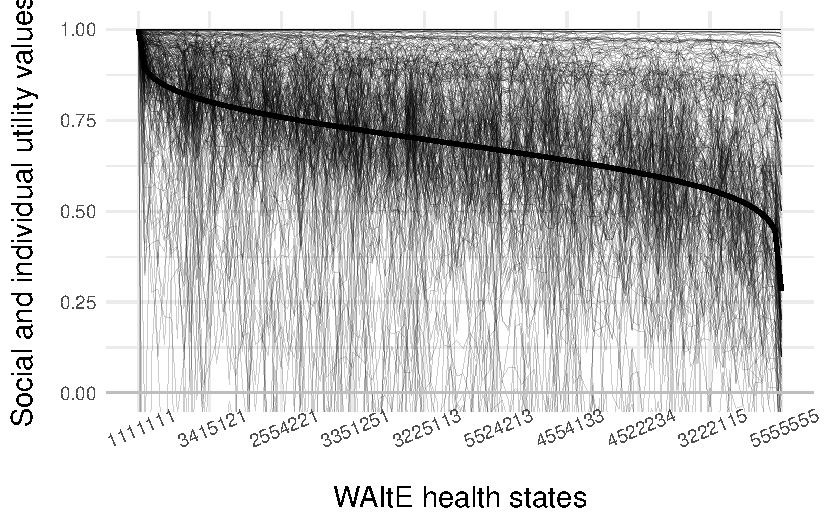
\includegraphics{quarto_files/figure-pdf/fig-sufplain-1.pdf}

}

\caption{\label{fig-sufplain}Social and individual utility functions}

\end{figure}%

\subsection{Preference heterogeneity}\label{preference-heterogeneity-1}

After estimating individual PUFs for all participants, pairwise EUD was
estimated between all participants. This yielded a {[}300 \(\times\)
300{]} distance matrix with 44,850 unique pairwise comparisons. The mean
(SD) and median (IQR) EUD were 115.7255744 (253.07) and 61.08 (33.17;
100.31). The highest and lowest observed EUD were 2150.75 and 0.
Figure~\ref{fig-eud} illustrates the relationship between EUD and WAItE
health states. EUD tends to increase as WAItE health states worsen. That
is, as the severity of WAItE health states increases, the more
heterogeneous preferences become among our sample.

\begin{figure}

\centering{

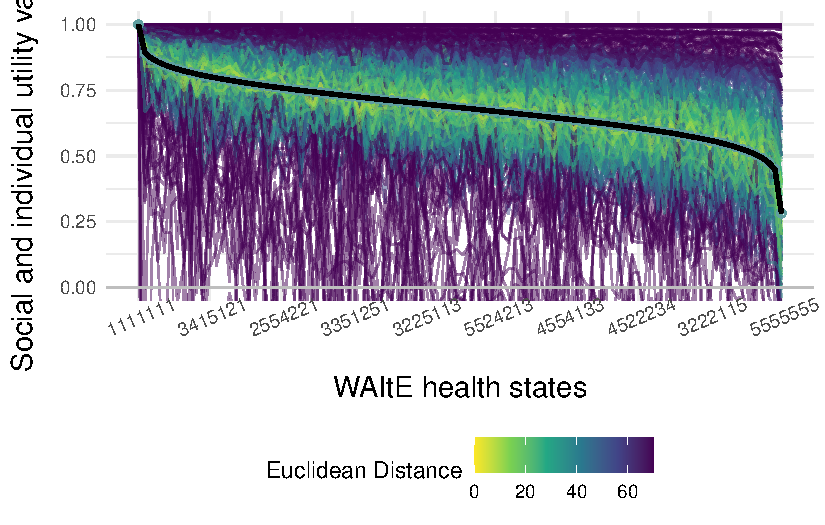
\includegraphics{quarto_files/figure-pdf/fig-eud-1.pdf}

}

\caption{\label{fig-eud}Social and individual utility functions coloured
by EUD}

\end{figure}%

\subsection{PERMANOVA}\label{permanova}

Table~\ref{tbl-permanova} presents the PERMANOVA model results.
Presented are within‐group sum‐of‐squares (SS\(_W\)) for each group
individually and for all groups combined, and the corresponding R\(^2\),
pseudo \(F\), and \(p\) values. Preference heterogeneity was
significantly affected by age (\(p\) = 0.03), though the amount of
variability in preferences that could be explained by age was relatively
small (R\(^2\)=5.7\%). Figure~\ref{fig-age} presents the difference in
preferences between different age groups. Generally, as age increases,
health state utility values for each given WAItE health state are
higher. That is, younger populations tend to place more disutility on
WAItE health problems than older populations. While weight status was
not significantly related to preference heterogeneity according to the
PERMANOVA model, given the WAItE is a weight-specific measure, it was
informative to explore the relationship between preferences and weight
status. Though not statistically significant, we can observe a
difference in preferences between normal weight and overweight
individuals in Figure~\ref{fig-weight}. For a given WAItE health state,
overweight individuals in our sample placed less disutility on that
state than did normal weight individuals.

\begin{longtable}[]{@{}lrrrrr@{}}

\caption{\label{tbl-permanova}Results of PERMANOVA -- testing for
differences in WAItE health state preferences between group
characteristics}

\tabularnewline

\toprule\noalign{}
Variable & df & \(SS_W\) & \(R^2\) & F & Pr(\textgreater F) \\
\midrule\noalign{}
\endhead
\bottomrule\noalign{}
\endlastfoot
Age & 6 & 663590.648 & 0.057 & 3.018 & 0.030 \\
Weight status & 1 & 6892.412 & 0.001 & 0.188 & 0.724 \\
Education & 5 & 33542.464 & 0.003 & 0.183 & 0.968 \\
Occupation & 7 & 290563.598 & 0.025 & 1.133 & 0.270 \\
Gender & 3 & 57313.577 & 0.005 & 0.521 & 0.361 \\
Ethnicity & 4 & 521334.829 & 0.045 & 3.557 & 0.056 \\
Residual & 273 & 10003165.515 & 0.864 & & \\
Total & 299 & 11576403.042 & 1.000 & & \\

\end{longtable}

\begin{figure}

\centering{

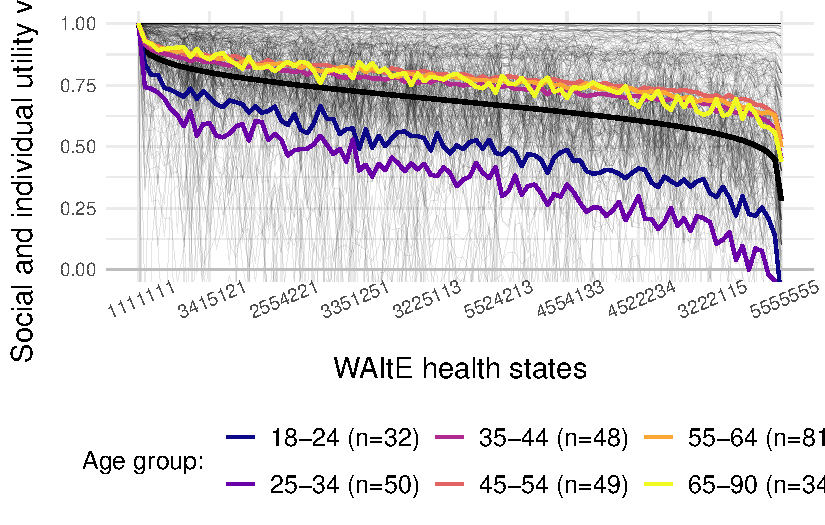
\includegraphics{quarto_files/figure-pdf/fig-age-1.pdf}

}

\caption{\label{fig-age}Social and individual utility functions grouped
by age status}

\end{figure}%

\subsection{Sensitivity analysis}\label{sensitivity-analysis-1}

EUD2 was estimated for each pairwise comparison of individuals in our
study. This yielded a {[}300 \(\times\) 300{]} distance matrix with
44,850 unique pairwise comparisons. The mean (SD) and median (IQR) EUD
were 34.30 (13.82) and 32.25 (24.54; 41.27). Results from the PERMANOVA2
analysis are presented in Table~\ref{tbl-permanova2}. After exclusion of
individual variation in anchoring responses, weight status and age had a
significant impact upon heterogeneity within our sample; though the
amount of heterogeneity that was explained by these variables was fairly
small (4.9\%).

\begin{longtable}[]{@{}lrrrrr@{}}

\caption{\label{tbl-permanova2}PERMANOVA2 -- testing for differences in
level rating and attribute weighting preferences between group
characteristics}

\tabularnewline

\toprule\noalign{}
Variable & df & \(SS_W\) & \(R^2\) & F & Pr(\textgreater F) \\
\midrule\noalign{}
\endhead
\bottomrule\noalign{}
\endlastfoot
Age & 6 & 8103.932 & 0.040 & 2.021 & 0.001 \\
Weight status & 1 & 1928.488 & 0.009 & 2.885 & 0.011 \\
Education & 5 & 4105.321 & 0.020 & 1.228 & 0.175 \\
Occupation & 7 & 4031.824 & 0.020 & 0.862 & 0.707 \\
Gender & 3 & 751.841 & 0.004 & 0.375 & 0.983 \\
Ethnicity & 4 & 3077.187 & 0.015 & 1.151 & 0.265 \\
Residual & 273 & 182464.444 & 0.892 & & \\
Total & 299 & 204463.039 & 1.000 & & \\

\end{longtable}

\begin{longtable}[]{@{}lrrrr@{}}

\caption{\label{tbl-glmpits}Multivariate Gamma GLM Model -- exploring
the relationship between PITS utility value and demographic
characteristics}

\tabularnewline

\toprule\noalign{}
& Estimate & Std. Error & t value &
Pr(\textgreater\textbar t\textbar) \\
\midrule\noalign{}
\endhead
\bottomrule\noalign{}
\endlastfoot
Intercept & 2.6957 & 0.0306 & 88.0719 & 0.0000 \\
Age & 0.0011 & 0.0004 & 3.0071 & 0.0029 \\
Education & -0.0007 & 0.0037 & -0.1858 & 0.8527 \\
Occupation & -0.0022 & 0.0023 & -0.9787 & 0.3285 \\
Gender & -0.0122 & 0.0107 & -1.1425 & 0.2542 \\
Ethnicity & 0.0059 & 0.0047 & 1.2677 & 0.2059 \\

\end{longtable}

\section{Discussion}\label{discussion}

This study is the first time that the OPUF has been used to estimate
health state utility values for the WAItE. We obtained a representative
sample of high quality data from Prolific, a survey company known for
their high quality respondents \citep{Peer2022DataResearch}. Our average
attribute weightings and implied ordering were similar to those
exhibited in Robinson et al.~(2024) \citep{Robinson2024AUKValue}.

Anchoring of the WAItE PITS state was a difficult procedure that
required a number of methodological decisions. We decided to use
uncensored responses to the Dead-VAS task which meant that data from one
respondent (-99) skewed the mean PITS utility value quite substantially.
To mitigate the impact of extreme values on the mean, we conducted
winsorization of values lying in the outer 0.1\% of the distribution.
This practice, while effective at limiting the influence of extreme
values on the mean, could understate the genuine variability in the
data. Though, it is likely that exclusion of this participant would have
had a more detrimental effect to presenting the genuine variability of
responses.

The social utility function elicited through this study, and underlying
utility value set, present monotonic preferences which behave as we
would have expected ex-ante (based on qualitative piloting work).
Tiredness and Unhappiness were considered the most important attributes
while Embarrassment and Sports the least. This finding concurs with
qualitative work conducted prior and also is in accordance with previous
valuation work done with the WAItE \citep{Robinson2024AUKValue}. Prior
valuation work, which used a DCE to elicit preferences, yielded latent
coefficients which violated the rational choice axiom of monotonicity.
In the OPUF, monotonicity is somewhat forced through the choice
architecture of the level rating and through the additional prompt to
reconsider responses that are not monotonic. Forced monotonicity, in
this context, could be problematic for eliciting unbiased preferences if
preferences for certain health states are truly not monotonic. For
example, prior qualitative work has suggested that ``I almost never get
tired'' might be preferable to ``I never get tired'' in some
circumstances where respondents are thinking about experiencing insomnia
and sleep quality. This being said, the WAItE descriptive system was
designed to be a monotonic descriptive system, validated using Rasch
analysis, and so having a monotonic utility value set makes logical
sense.

Preferences elicited through this study were considerably heterogeneous.
This can be understood through the mean EUD value (47.6) but also
illustrated in Figure~\ref{fig-sufplain} through the deviations of
individual PUFs from the social utility function. Following on from
prior work \citep{Schneider2024ExploringLevel}, we estimated EUD by
calculating a distance matrix between each pairwise comparison of
individual value sets for all 78125 WAItE health states. The implication
of estimating distance (preference heterogeneity) by using individual
value sets allows for much of the preference heterogeneity that exists
to be composed of differences in individual anchoring values (PITS state
responses) rather than differences in level ratings and attribute
weightings. This methodological decision, ultimately, results in the
majority of EUD being composed of differences in anchoring values and
this finding is important to acknowledge. Anchoring differences are
important to present and explore, though in this preference
heterogeneity analysis could be drowning out the heterogeneity in level
ratings and attribute weighting. An example of this can be shown through
the age preference heterogeneity in Figure~\ref{fig-age}. Preference
heterogeneity is evident between individuals above and below age 35 and
if we consider the mean PITS values for those two subgroups (age \(<\)
35 = -0.281; age \(>\) 34 = 0.487) we can see that a clear difference in
anchoring responses is evident.

A methodological exploration was conducted as a sensitivity analysis to
limit the influence that anchoring variation has on the overall
preference heterogeneity. We considered this to be a strength of the
research as it offers a new approach to decompose preference
heterogeneity into anchoring variation and the difference in level
ratings and attribute weightings. After exclusion of individual
variation in anchoring responses, weight status and age were found to
have a significant impact on preference heterogeneity within our sample;
though the amount of variation that could be explained was limited.
Preference heterogeneity between those of normal weight and those who
were overweight is illustrated in Figure~\ref{fig-weight}.

\begin{figure}

\centering{

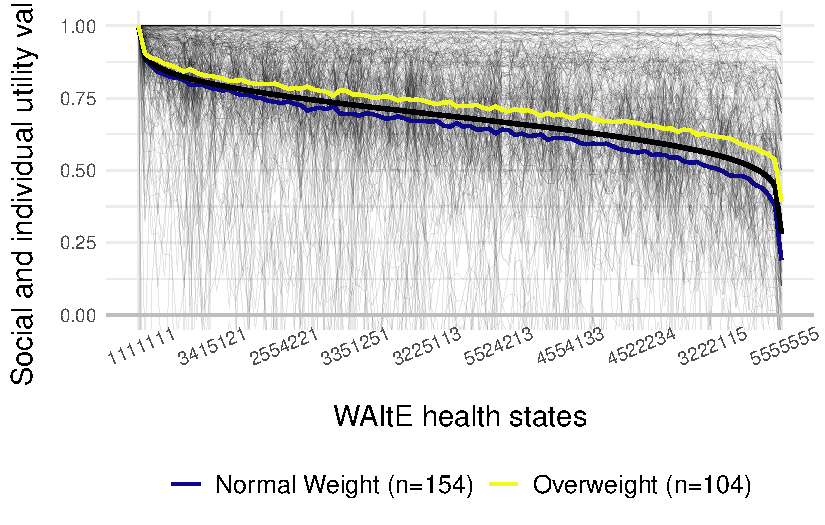
\includegraphics{quarto_files/figure-pdf/fig-weight-1.pdf}

}

\caption{\label{fig-weight}Social and individual utility functions
grouped by weight status}

\end{figure}%

This method of estimating preference heterogeneity should not be
considered the gold standard, as only part of the variation in
preferences is explored here. It can however be considered an additional
option for future researchers that wish to isolate the effect of
anchoring responses on overall preference heterogeneity. It is also, to
our knowledge, the first time preference heterogeneity has been
decomposed in this way with the OPUF.

The value set estimated here offers an alternative choice of preference
values to the existing value sets estimated using DCE (shown in
\citep{tab-WAItEvalsets}). When comparing the anchored coefficients
between value sets, one of the key areas of divergence is where levels
have been collapsed in the DCE value set. In the OPUF, ``I almost never
get tired'' is given 0.029 compared to 0.064 in the DCE due to
collapsing levels. Generally the difference between coefficients that
have not been `collapsed' between the value sets is small suggesting
that there is comparability to an extent between the value sets.
Anchoring values were broadly similar between studies too. The mean PITS
utility values between studies were broadly comparable with a maximum
range of 0.059. Interestingly, the EQ-VAS anchoring task mean (0.289)
was remarkably similar to the OPUF VAS anchoring task mean (0.282) again
supporting the use of VAS for elicitation of PITS utility values.

\begin{longtable}[]{@{}llll@{}}
\caption{Comparison of WAItE utility value sets}\tabularnewline
\toprule\noalign{}
Attribute.level & OPUF & DCE.TTO & DCE.VAS \\
\midrule\noalign{}
\endfirsthead
\toprule\noalign{}
Attribute.level & OPUF & DCE.TTO & DCE.VAS \\
\midrule\noalign{}
\endhead
\bottomrule\noalign{}
\endlastfoot
\textbf{Tired} & \textbf{} & \textbf{} & \textbf{} \\
Almost never & 0.029 & 0.064 & 0.059 \\
Sometimes & 0.052 & 0.064 & 0.059 \\
Often & 0.088 & 0.064 & 0.059 \\
Always & 0.14 & 0.148 & 0.137 \\
\textbf{Walking} & \textbf{} & \textbf{} & \textbf{} \\
Almost never & 0.021 & 0.015 & 0.013 \\
Sometimes & 0.045 & 0.015 & 0.013 \\
Often & 0.075 & 0.054 & 0.05 \\
Always & 0.116 & 0.106 & 0.098 \\
\textbf{Sports} & \textbf{} & \textbf{} & \textbf{} \\
Almost never & 0.012 & 0.021 & 0.019 \\
Sometimes & 0.023 & 0.021 & 0.019 \\
Often & 0.038 & 0.021 & 0.019 \\
Always & 0.069 & 0.058 & 0.053 \\
\textbf{Concentration} & \textbf{} & \textbf{} & \textbf{} \\
Almost never & 0.026 & 0.009 & 0.008 \\
Sometimes & 0.051 & 0.053 & 0.049 \\
Often & 0.08 & 0.067 & 0.062 \\
Always & 0.121 & 0.13 & 0.12 \\
\textbf{Embarrassment} & \textbf{} & \textbf{} & \textbf{} \\
Almost never & 0.012 & 0.007 & 0.007 \\
Sometimes & 0.022 & 0.025 & 0.023 \\
Often & 0.034 & 0.056 & 0.051 \\
Always & 0.061 & 0.069 & 0.064 \\
\textbf{Unhappiness} & \textbf{} & \textbf{} & \textbf{} \\
Almost never & 0.025 & 0.001 & 0.001 \\
Sometimes & 0.054 & 0.039 & 0.036 \\
Often & 0.083 & 0.076 & 0.07 \\
Always & 0.124 & 0.145 & 0.134 \\
\textbf{Treated differently} & \textbf{} & \textbf{} & \textbf{} \\
Almost never & 0.019 & 0.01 & 0.009 \\
Sometimes & 0.035 & 0.03 & 0.028 \\
Often & 0.052 & 0.075 & 0.069 \\
Always & 0.087 & 0.114 & 0.105 \\
\end{longtable}

\subsection{Appendix}\label{appendix}

\subsubsection{Derivation of EUD2}\label{sec-appendix1}

Matrices \(\tilde{M}_{1ij}\) and \(\tilde{M}_{2ij}\) denote latent
coefficient matrices from individual 1 and 2, for attributes \(i\) and
levels \(j\), from the analysis sample. Matrices \(\tilde{M}_{1ij}\) and
\(\tilde{M}_{2ij}\) were then anchored using the social PITS utility
value 0.282 (shown in Equation~\ref{eq-anchoring-matrices}).

\begin{equation}\phantomsection\label{eq-coef-1}{
\tilde{M}_{1ij} =  
\begin{bmatrix}
0 & 0 & 0 & 0 & 0 & 0 & 0 \\
0.03 & 0.02 & 0.01 & 0.01 & 0.02 & 0.03 & 0.05 \\
0.11 & 0.07 & 0.05 & 0.03 & 0.07 & 0.05 & 0.11 \\
0.15 & 0.09 & 0.07 & 0.04 & 0.12 & 0.08 & 0.19 \\
0.17 & 0.11 & 0.08 & 0.10 & 0.14 & 0.10 & 0.30
\end{bmatrix}
}\end{equation}

\begin{equation}\phantomsection\label{eq-coef-2}{
\tilde{M}_{2ij} =  
\begin{bmatrix}
0 & 0 & 0 & 0 & 0 & 0 & 0 \\
0.05 & 0.02 & 0.01 & 0.01 & 0.02 & 0.03 & 0.03 \\
0.15 & 0.11 & 0.03 & 0.05 & 0.09 & 0.04 & 0.09 \\
0.18 & 0.13 & 0.05 & 0.06 & 0.14 & 0.06 & 0.16 \\
0.21 & 0.15 & 0.06 & 0.11 & 0.17 & 0.08 & 0.23
\end{bmatrix}
}\end{equation}

\begin{equation}\phantomsection\label{eq-anchoring-matrices}{
    \tilde{V}_{1ij} = \tilde{M}_{1ij} \cdot (1-0.282); \quad
    \tilde{V}_{2ij} = \tilde{M}_{2ij} \cdot (1-0.282)
}\end{equation}

\begin{equation}\phantomsection\label{eq-vcoeff}{
\tilde{V}_{1ij} =  
\begin{bmatrix}
0.0 & 0.0 & 0.0 & 0.0 & 0.0 & 0.0 & 0.0 \\
0.02 & 0.01 & 0.01 & 0.01 & 0.01 & 0.02 & 0.04 \\
0.08 & 0.05 & 0.04 & 0.02 & 0.05 & 0.04 & 0.08 \\
0.11 & 0.06 & 0.05 & 0.03 & 0.09 & 0.06 & 0.14 \\
0.12 & 0.08 & 0.06 & 0.07 & 0.1 & 0.07 & 0.22
\end{bmatrix}
}\end{equation}

\begin{equation}\phantomsection\label{eq-vcoeff2}{
\tilde{V}_{2ij} =  
\begin{bmatrix}
0.00 & 0.00 & 0.00 & 0.00 & 0.00 & 0.00 & 0.00 \\
0.04 & 0.01 & 0.01 & 0.01 & 0.01 & 0.02 & 0.02 \\
0.11 & 0.08 & 0.02 & 0.04 & 0.06 & 0.03 & 0.06 \\
0.13 & 0.09 & 0.04 & 0.04 & 0.10 & 0.04 & 0.11 \\
0.15 & 0.11 & 0.04 & 0.08 & 0.12 & 0.06 & 0.17
\end{bmatrix}
}\end{equation}

Once anchored coefficient matrices Equation~\ref{eq-vcoeff} and
Equation~\ref{eq-vcoeff2} are estimated, a complete profile of health
state utility values for individual 1 and 2 are estimated for all 78,125
unique health states described by the WAItE. This yields a {[}78125
\(\times\) 1{]} vector for each individual ranging from (1, 0.282)
(shown in Equation~\ref{eq-healthstate-utilities}\}).

\begin{equation}\phantomsection\label{eq-healthstate-utilities}{
\begin{aligned}  
\tilde{U}_{1,s} &=  \{1, 0.98, 0.96, ..., 0.282\}; \quad \tilde{U}_{2,s} =  \{1, 0.97, 0.95, ..., 0.282\} \\
&\backepsilon \quad \quad s = \{1111111, 2111111, ..., 5555555\}
\end{aligned}
}\end{equation}

To estimate euclidean distance between the two health state utility
vectors, the square root of the sum of the squared differences between
each element in the vector is calculated (shown in
Equation~\ref{eq-EUD}, and populated for responses from individual 1 and
2 in Equation~\ref{eq-pairwiseEUD2}).

\begin{equation}\phantomsection\label{eq-EUD2}{
  \begin{aligned}
    d_{EUD2}(i,j) & =\sqrt{\sum_{}^{}(u_{i}(s_{1})-u_{j}(s_{1}))^{2}+ ... +(u_{i}(s_{78125})-u_{j}(s_{78125}))^{2}}\\
      & \backepsilon \quad \quad s = \{1111111, 2111111, ..., 5555555\}\\
  \end{aligned}
}\end{equation}

\begin{equation}\phantomsection\label{eq-pairwiseEUD2}{
d_{EUD2}(i,j) = \sqrt{\{(1-1)^2+(0.98-0.97)^2+(0.96-0.95)^2+ ... +(0.282-0.282)^2\}}
}\end{equation}

Pairwise EUD2 was estimated for all possible combinations of individuals
in our analysis sample. EUD2 was stored in a distance matrix of
dimensions {[}300 \(\times\) 300{]}, where coordinates {[}3,7{]}
represents the EUD2 between individual 3 and 7. The mean of the distance
matrix provides the overall measure of disimilarity/heterogeneity within
the analysis sample.


  \bibliography{bibliography.bib}



\end{document}
